% \documentclass[fontsize=12pt,headsepline, twoside,open=right,cleardoublepage=empty,paper=a4,listof=totoc,bibliography=totoc]{scrreprt}

\documentclass[fontsize=12pt,headsepline, twoside,cleardoublepage=empty,paper=a4,listof=totoc,bibliography=totoc]{scrbook}

\usepackage{header}
\setcapindent{0pt}
\author{Henry von Wichert}
\date{\today}
\title{Untersuchung von Sekundärelektronenemission an Mikroentladungen mittels Energiestrommessungen}
\subtitle{Subtitle}
\subject{Bachelorarbeit}

%Verwenden, wenn ohne Seitenumbrüche gearbeitet werden soll.
%\RedeclareSectionCommand[style=section,indent=0pt]{chapter}

\begin{document}
\makeatletter

%\frontmatter
\pagenumbering{roman}



%Einfügen der Titelseite
\begin{titlepage}
\cleardoublepage\pdfbookmark{Startseite}{title}
   
\begin{minipage}[t]{.6\linewidth} %
     \vspace*{0pt} {\Large Christian-Albrechts-Universität zu Kiel\\}
                Mathematisch-Naturwissenschaftliche Fakultät\\
                Institut für Experimentelle und Angewandte Physik\\
                Arbeitsgruppe Plasmatechnologie\\
\end{minipage}% 


\vspace*{4.2cm}

	{\Huge\begin{center}
		{\textbf{\@title}}
	\end{center}}

	\vspace{2.cm}
	
	\begin{center}
		{\large{\textbf{\@subject}}\\}
		\vspace{0.5cm}
	\end{center}

	\vspace{1cm}

	\begin{center}
		{\textbf{}}\\
		{\@author\\}
		\vspace{0.5cm}
		{\@date}
	\end{center}

	\vspace*{\fill}
	\pagestyle{empty}
	
	\begin{flushleft}
	    \begin{tabular}{l l}
            Erstgutachter: & Prof. Dr. ??\\
		    Zweitgutachter: & ??\\
        \end{tabular}
	\end{flushleft}
	

%%%%%%%%%%%%%%%%%%%%%%%%%%%%%%%%%%%%%%%%%%%%%%%%%%%%%%%%%%%%%%%%%%%%%%%%%%%%%%%	
% 	\newpage
% 	\begin{flushleft}
% 		\vspace*{\fill}
% 		\textbf{von \@author}\\
% 		\emph{}\\
% 		??, Christian-Albrechts-Universität zu Kiel, ??
% 	\end{flushleft}
%%%%%%%%%%%%%%%%%%%%%%%%%%%%%%%%%%%%%%%%%%%%%%%%%%%%%%%%%%%%%%%%%%%%%%%%%%%%%%%	
\end{titlepage}
\makeatother
%----------------------------------------------------------------------
%%%%%%%%%%%%%%%%%%%%%%%%%%%%%%%%%%%%%%%%%%%%%%%%%%%%%%%%%%%%%%%
%\thispagestyle{empty}
\pdfbookmark{Zusammenfassung}{zusammenfassung}
\noindent
\textbf{\huge \textsf{Zusammenfassung}}
	
	
\vspace{2\baselineskip}
	\noindent
	Bla Bla Bla
	%\newpage
	\cleardoublepage
%%%%%%%%%%%%%%%%%%%%%%%%%%%%%%%%%%%%%%%%%%	
%Hier ist die englische Zusammenfassung
%	\thispagestyle{empty}
% 	\pdfbookmark{Abstract}{abstract}
% 	\noindent
% 	\textbf{\huge \textsf{Abstract}}
	
% 	\vspace{2\baselineskip}
% 	\noindent
% 	Here the Abstract could be.
%\cleardoublepage
	
%-------------------------------------------------------------------------


%Inhaltsangabe
	\pdfbookmark{Inhalt}{toc}
	\tableofcontents
    \cleardoublepage

%Hauptteil
\pagenumbering{arabic}
%Und hier beginnt dann der Hauptteil	
%	\mainmatter


\chapter{Einleitung}

Plasmen dienen in vielen Bereichen der Wissenschaft und Technik nicht nur als Versuchsobjekt, sondern auch als Werkzeug. Besonders nützlich sind dabei die hohe Elektronentemperatur bei niedriger Gastemperatur in nicht-thermischen Plasmen, sowie die Möglichkeit, Ladungsträger im Plasma gerichtet zu beschleunigen \cite{liebermanPrinciplesPlasmaDischarges1994a,pielPlasmaPhysicsIntroduction2010,chenIntroductionPlasmaPhysics1984}. Die hohe Elektronentemperatur kann in plasmachemischen Verfahren zur effizienten Überwindung der Aktivierungsenergie einer Reaktion genutzt werden, während die gerichtete Beschleunigung zum Beispiel in der Oberflächenbearbeitung genutzt wird. So werden beim Sputtern Atome von einem Target durch die Ionen des Plasmas abgetragen und ins Plasma eingebracht. Diese können dann im Plasma ionisiert und schließlich auf eine Oberfläche aufgebracht werden. So können die Eigenschaften des Plasmas unter anderem zur Herstellung schützender Schichten auf Werkzeugen, antireflektiver Schichten auf Glasscheiben und funktionaler Schichten auf Solarzellen verwendet werden \cite{weltmannFuturePlasmaScience2019,martinHandbookDepositionTechnologies2009}. Solche Methoden benötigen typischerweise einen Niederdruck in der Größenordnung von wenigen Millibar, weshalb Vakuumkammern für diese Prozesse notwendig sind. Zur Einsparung dieser Vakuumanlagen und dadurch einfacheren Einbindnung in industrielle Prozesse ist die Verwendung von Atmosphärendruckplasmen für die Prozesstechnik interessant. Auch zur Erreichung höherer Durchsätze in plasmachemischen Prozessen sind die höheren Dichten bei Atmosphärendruck nützlich. Schon seit einiger Zeit wurden dafür geeignete Plasmaquellen entwickelt \cite{winterAtmosphericPressurePlasma2015,bruggemanFoundationsAtmosphericPressure2017,tenderoAtmosphericPressurePlasmas2006}. Mit dieser Technik lassen sich nicht nur bereits bekannte Verfahren vereinfachen, sondern auch neue Prozesse ermöglichen. Ein vielversprechendes Beispiel dafür ist die medizinische Behandlung von Wunden durch Plasmen \cite{vonwoedtkePlasmasMedicine2013,gravesLowTemperaturePlasma2014a}. Plasmen wirken dabei antibakteriell und desinfizierend \cite{schneiderRoleVUVRadiation2012}.\\

Wegen des Paschen-Gesetzes sind zum Zünden von Atmosphärendruckplasmen hohe Spannungen nötig. Daher erfordert der stabile Betrieb einer solchen Entladung andere Ansätze \cite{bruggemanFoundationsAtmosphericPressure2017}. Einer dieser Ansätze ist die Miniaturisierung der Entladung in einem Mikroplasma \cite{bruggemanAtmosphericPressureDischarge2013}. Solche Entladungen ermöglichen die Zündung einer relativ kalten Glimmentladung bei Elektrodenabständen um die \qty{100}{\um}. Eine solche Entladung wird in dieser Arbeit untersucht.\\

In der Forschung an Atmosphärendruckplasmen gibt es noch viele offene Fragen. So sind bei bestimmten Prozessen Modellrechnungen nur bei Niederdruck möglich, da es bei Normaldruck deutlich mehr Stöße mit Gasteilchen gibt, die in Modellen nur schwer zu berücksichtigen sind. Einer dieser Prozesse ist die Sekundärelektronenemission, also das Phänomen, dass energiereiche Teilchen beim Aufprall auf eine Oberfläche Elektronen aus dieser herausschlagen können \cite{arumugamEffectiveSecondaryElectron2017}. Ziel dieser Arbeit ist es, durch Energiestrommessungen an einer Mikroentladung das Maß zu bestimmen, in dem die Emissionsrate der Sekundärelektronen mit dem Strom der Ionen auf die Kathode zusammenhängt.
\chapter{Theorie}


\section{Der Plasmazustand}

Die üblichen drei Aggregatszustände sind nach der Energie und \glqq{}Freiheit\grqq{} der Teilchen geordnet. Führt man zum Beispiel Energie einem Festkörper zu, brechen die festen Bindungen zwischen den einzelnen Atomen oder Molekülen, die die Struktur des Festkörpers erhalten, und die Teilchen sind nur noch schwach aneinander gebunden. Die Substanz ist nun flüssig. Gibt man dieser Flüssigkeit noch mehr Energie zu, lösen sich auch die schwächeren Verbindungen. Die Teilchen sind dann völlig unabhängig voneinander und bilden ein Gas. Führt man dem Gas noch weitere Energie zu, lösen sich die äußersten Elektronen teilweise von ihren Atomrümpfen und es bildet sich ein \textit{Plasma}. 

Die Bezeichnung \glqq{}Plasma\grqq{} wurde 1928 von Irving Langmuir eingeführt, den der Transport der freien Ladungsträger in der Entladung an den Transport von roten und weißen Blutkörperchen im Blutplasma erinnerte \cite{langmuirOscillationsIonizedGases1928,hirshGaseousElectronics2012}.

\subsection{Allgemeine Eigenschaften eines Plasmas}

Zur Beschreibung von Gasen ist es ausreichend, nur die lokalen Stöße zwischen den Teilchen zu betrachten, wie es in der kinetischen Gastheorie geschieht \cite{feynmanrichardpFeynmanLecturesPhysics1964}. Bei einem Plasma ist es dagegen nicht möglich, neutrale Teilchen, Atomrümpfe und Elektronen als separate, herkömmliche Gase zu beschreiben. Der hauptsächliche Unterschied zwischen Gas und Plasma liegt im kollektiven Verhalten \cite{pielPlasmaPhysicsIntroduction2010}. Während die Van-der-Waals-Wechselwirkungen zwischen Gasmolekülen mit $ r^{-6} $ so schnell abklingen, dass die Stoßbeschreibung ausreicht, wirkt die elektrische Kraft, die mit $ r^{-2} $ abklingt, als Fernwirkung zwischen Teilchen an verschiedenen Orten. Die Dominanz dieser elektrischen Wirkungen über die Stöße zwischen den Teilchen unterscheidet Gas und Plasma.

\subsubsection{Quasineutralität und Abschirmung}

Das Plasma als Ganzes ist elektrisch neutral, obwohl positive und negative Ladungsträger im Plasma frei voneinander vorhanden sind. Betrachtet man also ein hinreichend großes Volumen innerhalb des Plasmas, ist die Anzahl positiver und negativer Ladungsträger in etwa gleich.\footnote{Bzw. gewichtet mit den Ladungen der Ladungsträger im Falle mehrfacher Ionisation.} Dies ist durch die elektrischen Fernwirkungen im Plasma bedingt. Befänden sich beispielsweise in einer Gegend mehr positive als negative Ladungen, würden positive Ladungen von der Ladung abgestoßen und negative Ladungen angezogen. Es stellt sich ein Ausgleich der Raumladung ein.

Die Größenordnung, ab der ein Plasmavolumen groß genug ist, um Quasineutralität zu zeigen, wird durch die \textit{Debyelänge} gegeben. Wird eine äußere Ladung ins Plasma eingebracht, zieht diese ungleichnamige Ladungen aus dem Plasma an. Um die eingebrachte Ladung bildet sich dann eine Raumladungszone entgegengesetzter Ladung, die das Feld abschirmt. Diese Abschirmung geschieht exponentiell mit der Debyelänge $\lambda_{De,Di}$ als Skalenfaktor. Diese ist für Elektronen und Ionen (jeweils durch $ e $ bzw. $ i $ im Index gekennzeichnet) separat zu berechnen, da diese unterschiedliche Temperaturen $ T_{e,i} $ haben können. Dabei gilt \cite{pielPlasmaPhysicsIntroduction2010}
\begin{align*}
	\lambda_{De,Di}  = \sqrt{\dfrac{\epsilon_0k_BT_{e,i}}{n_{e,i}e_0^2}},
\end{align*}
wobei $ \epsilon_0 $ die elektrische Feldkonstante, $ k_B $ die Boltzmannkonstante, $ n_{e,i} $ die entsprechende Dichte und $ e_0 $ die Elementarladung bezeichnen.
Zusammenfassend kann man dann die sogenannte linearisierte Debyelänge $ \frac{1}{\lambda_D^2} = \frac{1}{\lambda_{De}^2} + \frac{1}{\lambda_{Di}^2} $ bilden. Um ein Plasma mit Quasineutralität zu gewährleisten, müssen sich in einer Kugel mit der Debyelänge als Radius viele Teilchen befinden \cite{pielPlasmaPhysicsIntroduction2010}: $ n\cdot\lambda_{D}^{3}\gg 1 $

\subsubsection{Zeitskala der elektrischen Wirkungen}

Der Ausgleich von Raumladungszonen im Plasma geschieht wegen des Impulses der Elektronen durch Einschwingen. Die Elektronen können also als Ensemble Schwingungen vollführen, welche die \textit{Plasmafrequenz} $ \omega_{P} $ haben. Eine analoge Plasmafrequenz lässt sich auch für die Ionen aufstellen \cite{pielPlasmaPhysicsIntroduction2010}:
\begin{align*}
	\omega_{Pe,Pi} = \sqrt{ \dfrac{n_{e,i} e_0^2}{\epsilon_0m_{e,i}}}
\end{align*}
Dabei ist $ m_{e,i} $ die Elektronen- bzw. Ionenmasse.
Eine zweite Zeitskala wird durch die Stoßfrequenz $ \nu $ gegeben, die beschreibt, wie häufig ein bestimmtes Teilchen mit anderen kollidiert. Die Dominanz der elektrischen Wirkungen über die normale Gaskinetik zeigt sich dann darin, dass die Plasmafrequenz in einem Plasma deutlich höher ist, als die Stoßfrequenz der Teilchen.

\subsubsection{Thermische und nicht-thermische Plasmen}

Die verschiedenen Spezies der Elektronen und Ionen sind in einem Plasma oft nicht im  thermodynamischen Gleichgewicht. Dies liegt daran, dass die Elektronen viel leichter sind als die Ionen und deshalb durch das elektrische Feld deutlich schneller und auf höhere Energien beschleunigt werden. Da beim Stoß eines leichten Elektrons mit einem schweren Ion jedoch nur sehr wenig Energie an das Ion übertragen wird, dauert eine Thermalisierung sehr lange. Die Ionen können, trotz der hohen Elektronentemperatur, als \glqq{}Teilgas\grqq{} deshalb deutlich kälter sein. Bei den in dieser Arbeit betrachteten Plasmen erhitzen sich die Elektroden zum Beispiel nur auf ca. 70-80\Grad C, was eine ähnlich niedrige Ionen- und Neutralgastemperatur impliziert.

Während die in dieser Arbeit betrachtete Glimmentladung damit ein nicht-thermisches Plasma ist, gibt es auch thermische Plasmen wie z.B. Lichtbogenentladungen, bei denen Elektronen- und Ionentemperatur im Gleichgewicht sind \cite{keudellVorlesungsskriptEinfuhrungPlasmaphysik2008}.



\subsection{Das Paschen-Gesetz und der Zündprozess}

Das Paschen-Gesetz beschreibt die Zündspannung eines Plasmas abhängig von Druck $ p $ und vom Abstand der Elektroden $ d $:
\begin{align*}
	U = B \cdot \dfrac{pd}{C + \ln pd}
\end{align*}
Dabei sind $ A $  und $ B $ gasspezifische Konstanten, $ C = \ln\frac{A}{\ln(1+1/\gamma_I)} $ und $ \gamma_I $ — die Anzahl der Sekundärelektronen, die ein Ion auf der Kathode im Durchschnitt direkt herauslöst — eine Materialkonstante.  

Dass die Zündspannung nach dem Paschen-Gesetz nur vom Produkt $ p\cdot d $ abhängt, liegt am Mechanismus des Durchbruchs.
Während der Zündung werden freie Elektronen von der angelegten Spannung beschleunigt, welche dann Atome ionisieren können und so durch die Produktion weiterer Elektronen eine Elektronenlawine erzeugen. Diese führt schließlich zur Ausbildung eines Plasmakanals. Dafür ist es wichtig, dass ein Elektron auf dem Weg zwischen zwei Stößen so sehr beschleunigt wird, dass es beim nächsten Stoß wieder ein Atom ionisieren kann. Da bei einem höheren Druck die freie Weglänge der Elektronen zwischen den Atomen kleiner ist, ist die erreichte Energie proportional zu $ 1/p $. Gleichzeitig ist die beschleunigende Feldstärke bei gegebener Spannung an den Elektroden proportional zu $ 1/d $. Insgesamt ist also die erreichte Energie und damit auch die nötige Zündspannung eine Funktion des Produkts $ pd $.

\begin{figure}[H]
	\centering
	\includesvg[width=0.85\linewidth]{plots/paschen_kurve}
	\caption{Die Paschenkurven von Helium, Argon und Luft bei \qty{1e5}{\pascal}. Die theoretischen Zündspannungen bei der Elektrodenentfernung von \qty{100}{\um} sind angeschrieben. (Konstanten A = \qty{2,25}{Pa^{-1}.m^{-1}}  ,B = \qty{25,5}{V.Pa^{-1}.m^{-1}} und $ \gamma =$ \num{0,1} aus \cite{lehrElectricalBreakdownGases2017,bohmRetardingfieldAnalyzerMeasurements1993}.)}
	\label{fig:paschen_kurve}
\end{figure}

Wie in Abb. \ref{fig:paschen_kurve} erkennbar, steigt für große $ pd $ die nötige Zündspannung an, zum Beispiel, wenn der Elektrodenabstand sehr groß wird. Bei kleineren $ pd $ erreicht diese sogenannte \textit{Paschen-Kurve} zunächst ein Minimum und steigt dann für noch kleinere $ pd $ stark an. Da bei hohen Zündspannungen viel Strom fließt und einen Lichtbogen erzeugt, ist es für Glimmentladungen in Helium als Arbeitsgas notwendig, möglichst nah am Minimum der Paschen-Kurve zu arbeiten. Dieses tritt bei einem konstanten $ pd $-Produkt auf  \cite{paschenUeberFunkenuebergangLuft1889,rajzerGasDischargePhysics1997}.

Um die minimale Zündspannung zu ermöglichen, muss deshalb der Abstand der Elektroden bei höherem Druck stark verringert werden. In dieser Arbeit werden die Elektroden \qty{100}{\um} voneinander entfernt gehalten. Damit ist der Abstand noch deutlich über dem Paschenminimum von etwa \qty{30}{\um} oder sogar \qty{6}{\um} bei Argon (siehe Abb. \ref{fig:paschen_kurve}). Dies ist in der Praxis aber üblich, da sehr kleine Elektrodenentfernungen nur schwer zu realisieren sind \cite{bruggemanFoundationsAtmosphericPressure2017}.

\subsection{Mikroplasmen}

Plasmen, die auf einer Skala von \qty{1}{\um} bis \qty{1}{\mm} betrieben werden, werden als Mikroplasmen bezeichnet \cite{edenMicrocavityPlasmaDevices2005}. Um bei so kleinen Elektrodenabständen ein Plasma zu zünden, werden Drücke in der Größenordnung des Atmosphärendrucks von etwa \qty{1e5}{\Pa} benötigt. In Abbildung \ref{fig:paschen_kurve} ist gut erkennbar, dass das Paschen-Minimum bei Atmosphärendruck in diese Größenordnung des Elektrodenabstandes fällt. Zusätzlich zum Betrieb bei oder sogar über Atmosphärendruck haben Mikroplasmen noch viele weitere interessante Eigenschaften, welche sich teilweise in dieser Arbeit beobachten lassen. Besonders die hohe Leistungsdichte, die sich in solchen Plasmen ergibt, lässt sich in einer größeren Entladung nur schwer erreichen. Beispielsweise wird die Leistungsdichte des hier betrachteten Mikroplasma auf \qty{3e4}{W.cm^{-3}} geschätzt.\\

Der Betrieb von Mikroplasmen ist in vielen verschiedenen Elektrodengeometrien möglich. So können zum Beispiel Hohlräume der entsprechenden Größenordnung auf der Kathode verwendet werden \cite{dzikowskiElectricFieldStrengths2022}. Auch das flächige Plasma einer dielektrisch behinderten Oberflächenentladung (SDBD) ist aus einzelnen Mikroplasmen aufgebaut \cite{hoderComplexInteractionSubsequent2017}. Die wohl einfachste Elektrodengeometrie mit der ein Mikroplasma gezündet werden kann, sind zwei parallele, ebene Elektroden. Anders als z.B. bei dielektrisch behinderten Entladungen kann ein Plasma so mit Gleichstrom betrieben werden. Deshalb und aufgrund der Einfachheit des Aufbaus wird in dieser Arbeit eine solche Entladung untersucht.

\section{Passive Thermosonden}
Die passive Thermosonde (PTP) und ihr Messprinzip gehen auf eine Arbeit von Thornton \cite{thorntonSubstrateHeatingCylindrical1978} im Jahre 1978 zurück. 
Passive Thermosonden ermöglichen die Messung von Energieströmen im Plasma, indem sie die Erwärmung eines Testkörpers messen. Da diese Sonden einfach zu verstehen und bauen sind, werden sie in der Plasmaphysik häufig zur Diagnostik benutzt \cite{benediktFoundationsMeasurementElectrons2021,gauterCalorimetricProbeMeasurements2017,rosenfeldtUsePassiveThermal2021a}.
Die Heizleistung ergibt sich als Bilanz vieler einzelner Energieströme auf die Sonde, zum Beispiel der Heizung durch Ladungsträger, Neutralteilchen und Strahlung, abgeführte Energie durch Sekundärelektronenemission und der Energiebilanz von Rekombinationsprozessen auf der Sondenoberfläche. 
%In Kombination mit anderen diagnostischen Verfahren kann der gesamte Energiestrom dann in die Komponenten aufgeschlüsselt werden.

\subsection{Aufbau der Sonde}
Der Sondenkopf besteht aus einem Dummy-Plättchen, das die Leistung des Plasmas aufnimmt. An dieses Plättchen sind durch Punktschweißen ein Typ-K Thermoelement und ein Kupferdraht befestigt \cite{haaseDynamicDeterminationSecondary2018}. Zur thermischen Isolierung des Plättchens steht dieses frei und ist nur über die Drähte befestigt \cite{kewitzInvestigationCommercialAtmospheric2015,cipoDiagnosticsProcessPlasma2020}. Über das Thermoelement kann der Temperaturverlauf des Sondenplättchens aufgezeichnet werden. Der Kupferdraht dient als elektrische Verbindung, die hier zum Zünden des Plasmas genutzt wird. Durchmesser und Dicke des Plättchens sind vom jeweiligen Aufbau abhängig. Je nach Größe und Leistung des Plasmas kann ein passender Durchmesser genutzt werden. Da in dieser Arbeit an einem Mikroplasma mit geringer Leistung gemessen wird, werden 5mm große Plättchen genutzt. Um eine empfindlichere Messung bei geringen Energieströmen zu erreichen, wird die Wärmekapazität des Plättchens mit einer Dicke von \qty{100}{\um} klein gehalten.
%?????

\subsection{Messprinzip}\label{messprinzip}

Die Energiebilanz des Substrats wird durch dessen Enthalpie $ H $ und deren Änderung $ \dot{H} $ beschrieben. Dabei ist $ \dot{H} $ die Bilanz der Leistung $ P_\text{in} $ an das und $ P_\text{out} $ von dem Substrat, vorausgesetzt es gibt keine Prozesse innerhalb des Plättchens. Über die Wärmekapazität $ C $ des Substrats ist die Änderung der Enthalpie mit der der Temperatur verbunden \cite{gauterCalorimetricInvestigationPlasma2018}
\begin{align*}
\dot{	H} = C \dot{T} = P_\text{in} - P_\text{out}.
\end{align*}
Wird das Plasma angeschaltet, heizt dieses das Plättchen. Gleichzeitig gibt es durch verschiedene Mechanismen eine  Abfuhr von Wärme aus dem Substrat, die unter $ P_\text{out} $ zusammengefasst wird. Wird nun das Plasma ausgeschaltet, fällt der heizende Wärmestrom weg und das Plättchen kühlt ab. Die Änderung der Enthalpie können wir mit zwei Gleichungen beschreiben \cite{gauterCalorimetricInvestigationPlasma2018}:
\begin{align*}
	\text{Heizen:}\quad \dot{H}_h &= C \dot{T}_h = P_\text{in} - P_{\text{out},h}\\
	\text{Kühlen:}\quad \dot{H}_c &= C \dot{T}_c =- P_{\text{out},c}
\end{align*}

Unter der Annahme, dass die abgeführte Leistung $ P_\text{out} $ nur von der Temperatur abhängig ist und nicht davon, ob das Plasma an- oder ausgeschaltet ist, kann $ P_\text{in} $ durch Vergleich beider Temperaturänderungen bestimmt werden \cite{thorntonSubstrateHeatingCylindrical1978}
\begin{align*}
	P_\text{in} = C( \dot{T}_h - \dot{T}_c).
\end{align*}

\subsection{Auswertungsmethodik}


Um eine Veränderung der Rahmenbedingungen während der Messung zu vermeiden, wird das Plasma dazu nur kurz (hier \qty{10}{\second}) angeschaltet, sodass zwischen den Messungen des Heizens und Abkühlens wenig Zeit vergeht und $ P_\text{out} $ als in beiden Fällen identisch angenommen werden kann. Die Messdaten sind dann Reihen solcher Aufheiz- und Abkühlphasen, die durch das Ein- und wieder Abschalten des Plasmas erzeugt werden. Im Temperaturverlauf der Sonde zeigen sich diese als Temperaturspitzen (siehe Abb. \ref{fig:peask_bsp}). Zur Auswertung der Daten wird hier die \textit{dT-Methode} \cite{rosenfeldtUsePassiveThermal2021,gauterCalorimetricInvestigationPlasma2018,hansenEnergyFluxMeasurements2019,hansenUnderstandingEnergyBalance2021} verwendet, die im Folgenden erklärt wird.\\

Bei konstanter Eingangsleistung kann man zeigen, dass die resultierende Temperaturkurve einem exponentiellen Verlauf folgt \cite{gauterCalorimetricInvestigationPlasma2018}:

\begin{align*}
	T_h(t) &= T_{eq} + \dfrac{P_\text{in}}{\alpha} - \left( \dfrac{P_\text{in}}{\alpha} \right) \exp\left( - \dfrac{\alpha}{C}t \right)\\
	T_c(t) &= T_{eq} + (T_{st} - T_{eq}) \exp\left( - \dfrac{\alpha}{C}t \right)
\end{align*}
Dabei ist $ T_{eq} $ die Gleichgewichtstemperatur, auf die das Plättchen ohne Plasma abkühlt, $ T_{st} $ die Temperatur am Anfang des Abkühlens und $ \alpha $ eine Konstante des Plättchens, die die Effizienz des Abkühlens beschreibt. Aufgrund des exponentiellen Charakters des Verlaufs, gibt es einen linearen Zusammenhang zwischen der Substrattemperatur und deren Ableitung.
\begin{align*}
 	\dfrac{\dd T_h}{\dd t} &= - \dfrac{\alpha}{C} \cdot T_h  + \dfrac{\alpha T_{eq} + P_\text{in}}{C}\\
 	\dfrac{\dd T_c}{\dd t} &= - \dfrac{\alpha}{C} \cdot T_c  + \dfrac{\alpha T_{eq}}{C}\\
\end{align*}

Dabei ist die Steigung für eine bestimmte Sonde konstant. Die Differenz der konstanten Terme ist dann proportional zur Heizleistung.
\begin{figure}[h]
	\centering
	\includesvg[width=\linewidth]{plots/peak_bsp}
	\caption{\textbf{a)} Beispielhafte Darstellung eines Temperaturpeaks. \textbf{b)} Der selbe Temperaturpeak in dT-Darstellung. Es werden lineare Fits an die linearen Bereiche gezeigt, deren Steigungen nahezu parallel sind.}
	\label{fig:peask_bsp}
\end{figure}

Trägt man wie in Abb. \ref{fig:peask_bsp} die Temperaturänderung gegen die Temperatur auf, erkennt man diese zwei linearen Bereiche, die dem Heiz- und Kühlprozess entsprechen. Beide zeigen die gleiche Steigung, die Heizkurve liegt jedoch in der Grafik oben. Durch lineare Regression lassen sich die beiden Kurven vergleichen. In der Theorie ergibt sich die Leistung einfach aus der Differenz der Achsenabschnitte multipliziert mit der Wärmekapazität der Sonde. Da die Steigungen in der Praxis jedoch fehlerbehaftet und nicht exakt gleich sind, wird die Differenz in der Mitte der Regressionsbereiche gebildet. Bei einer Differenzbildung der y-Achsenabschnitte hätte der Unterschied der Steigungen einen größeren Einfluss als nötig, da sich dieser außerhalb der Bereiche verstärkt.


\paragraph{Glättung der Datenreihe}
Um die Ableitung einer verrauschten Datenreihe zu bilden, ist es wichtig, die Daten vorher zu glätten, da die Differenzenbildung aufeinanderfolgender Werte das Rauschen in den Daten verstärkt. Dabei hat die Methode der Glättung einen großen Einfluss darauf, wie viel geglättet werden muss, um eine saubere Ableitung berechnen zu können. Dies liegt an den Eigenschaften der Faltung. Die Ableitung der Faltung einer Funktion mit einem Faltungskern ist gleich der Faltung der Funktion mit der Ableitung des Kerns \cite{forsythdavidComputerVisionModern2012}
\begin{align*}
	\dfrac{\dd }{\dd x} (f*k)(x) = f*\left(\!\dfrac{\dd k}{\dd x}\right).
\end{align*}
Eine einfache Glättung durch einen laufenden Mittelwert entspricht der Faltung mit einem rechteckigen Faltungskern der Länge $ l $ des Glättungsfensters. Damit entspricht die Ableitung der so geglätteten Funktion der Faltung mit einem Kern der Form
\begin{align*}
	\dfrac{\dd k}{\dd x} = \dfrac{1}{l} \left(\delta\left(x+ \dfrac{l}{2}\right) -\delta\left(x- \dfrac{l}{2}\right)\right).
\end{align*}
Die so berechnete Ableitung wäre also wieder nur die Differenz zweier einzelner Datenpunkte, die hier nur weiter auseinanderlägen.

Dieses Problem kann mit einer Methode aus dem Feld der automatischen Bildverarbeitung und -erkennung gelöst werden, da auch für die Kantenerkennung in Bildern die Ableitung von verrauschten Daten gebildet werden muss. Anstatt eines Rechteckfensters wird hier eine Gaußkurve zum Glätten verwendet \cite{forsythdavidComputerVisionModern2012,dengAdaptiveGaussianFilter1993}. Bei der Ableitung einer so geglätteten Kurve werden die Differenzen der Werte ganzer Bereiche gebildet, da die Ableitung der Gaußkurve nicht nur zwei Spitzen hat. Dies führt dazu, dass die so abgeleiteten Daten wesentlich weniger verrauscht sind, wie in Abb. \ref{fig:gaussglaettung} sichtbar wird. Zudem wird der Einfluss einzelner Ausreißer in den Daten verringert, sodass diese nicht zu abrupten Sprüngen in der Ableitung führen.
Um die Daten nicht übermäßig zu glätten, wird für die Gaußkurve hier eine Standardabweichung von 10 Datenpunkten, also $ \frac{1}{9} $ s, genutzt.

\begin{figure}[p]
\centering
\includesvg[width=0.96\linewidth]{plots/gaussglaettung}
\caption{Vergleich zwischen gaußartiger Glättung und laufendem Durchschnitt:\textbf{a)} Ungeglättete Datenreihe; \textbf{b,c)} Glättungskerne beider Art und deren Ableitungen. Beide Kerne haben die gleiche Standardabweichung. Die Ableitung des Gaußkerns ist zur besseren Sichtbarkeit vertikal vergrößert. In Grau: Ausschnitt aus dem Rohsignal als Beispiel; \textbf{d,e)} Mit den jeweiligen Kernen geglättetes Signal; \textbf{f,g)} Die Ableitungen der entsprechenden Signale; \textbf{h,i)} Die beider Art geglätteten Signale in dT-Darstellung.}
\label{fig:gaussglaettung}
\end{figure}

Beim Vergleich beider Methoden zeigt sich, dass ein Gaußkern zu einem deutlich rauschfreieren Ergebnis führt als eine Glättung mit einem Rechteckkern gleicher Standardabweichung. Trotzdem führen Ausreißer in den Daten weiterhin zu Schwankungen in der Ableitung. In der linearen Regression werden jedoch die Quadrate der Fehler betrachtet. Die Abweichung hat deshalb weniger Einfluss auf das Regressionsergebnis, wenn der Fehler anteilig auf aufeinanderfolgende Datenpunkte aufgeteilt wird, anstatt eine große Abweichung in einem einzelnen Datenpunkt zu verursachen.

\subsection{Kalibierung der Sonde}

Eine der größten Schwierigkeiten bei der Benutzung passiver Thermosonden ist deren Kalibrierung, also die Bestimmung der Wärmekapazität des Sondenkopfes. Diese funktioniert nach dem in \cite{stahlCalorimetricProbePlasma2010a} beschriebenen Verfahren. Durch die Bestimmung des Volumens des Substratplättchens lässt sich ein Schätzwert der Wärmekapazität erhalten. Bei einem Kupferplättchen mit Durchmesser 5mm und Dicke \qty{100}{\um} ergibt sich ein Wert von \qty{0,0068}{\joule\per\kelvin}. Dies ist jedoch nicht der einzige Beitrag zur Wärmekapazität der Sonde, da das Plättchen mit einem Draht verbunden ist, welcher zusätzlich Kontakt zum Rest der Sonde hat. Obwohl sich bei einer kurzen Heizung des Plättchens nicht die ganze Sonde thermalisiert, lässt sich durch Messung an einer bekannten Quelle eine effektive Wärmekapazität bestimmen. Diese liegt meistens bei etwa \qty{0,01}{\joule\per\kelvin} und damit deutlich über der Wärmekapazität des einzelnen Plättchens. Hier wird als Wärmequelle ein Elektronenstrahl genutzt, der bei bekannter Leistung für \qty{30}{\second} die Sonde heizt. Die Wärmekapazität lässt sich dann aus der Temperaturänderungsrate und der Leistung des Strahls errechnen.

\section{Sekundärelektronenemission (SEE)}
Energiereiche Teilchen können beim Aufprall auf ein Substrat Elektronen aus diesem herauslösen. Dafür müssen die Teilchen genug Energie an ein gebundenes Elektron geben, sodass dieses die nötige Austrittsarbeit überwinden kann. Dies kann beim Stoß eines energiereichen Teilchens auf die Oberfläche geschehen, oder als separate Energieabgabe, wie bei der Abregung metastabiler Teilchen auf der Oberfläche.
\subsection{Der Sekundärelektronenemissionskoeffizient (SEEC)}
Der Sekundärelektronenemissionskoeffizient $ \gamma $ gibt an, wie viele Elektronen ein einfallendes Ion im Mittel aus der Kathode löst. Dabei ist es wichtig zu betrachten, durch welchen Mechanismus ein Sekundärelektron emittiert wird. Einige dieser Emissionsmechanismen werden in Abb. \ref{fig:see} dargestellt. Werden nur Sekundärelektronen betrachtet, die tatsächlich und direkt durch den Aufprall von Ionen herausgelöst werden, ergibt sich der Koeffizient $ \gamma_I $, der bei etwa \numrange{0,01}{0,1} liegt \cite{mariottiExperimentalStudyBreakdown2004}. 
\begin{figure}[h]
	\centering
	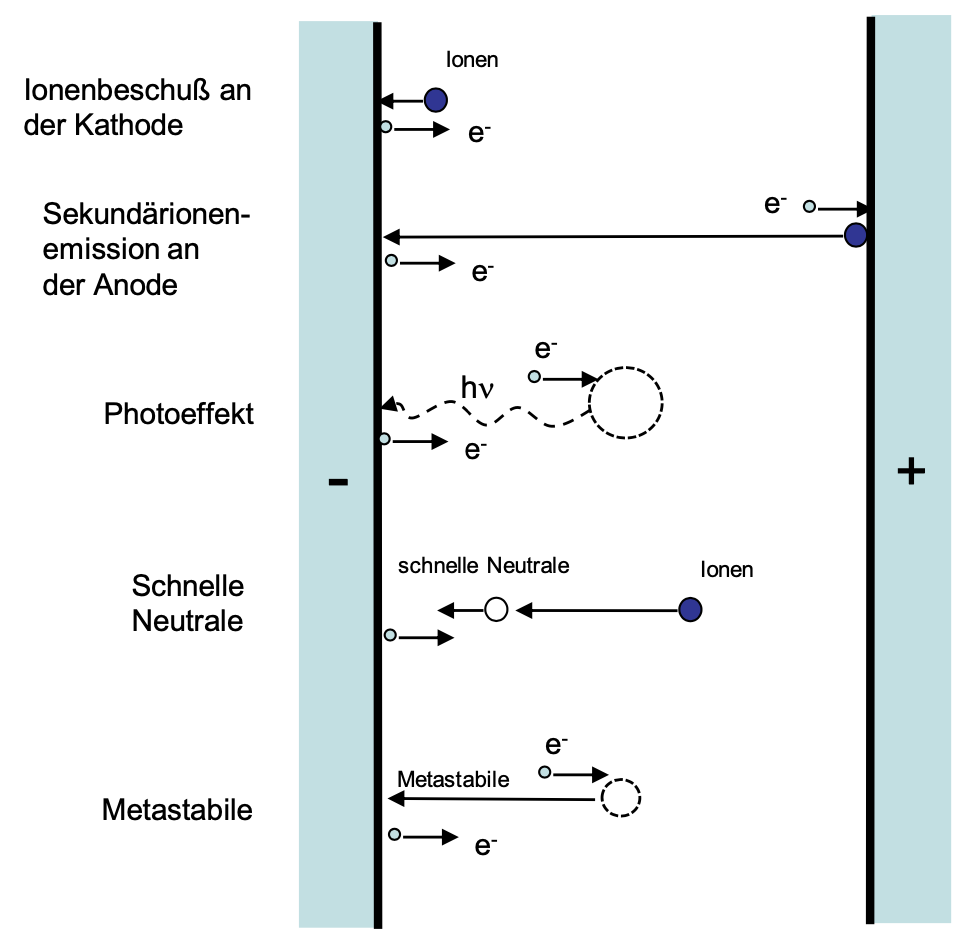
\includegraphics[width=0.7\linewidth]{bilder/see}
	\caption{Die verschiedenen Mechanismen der Sekundärelektronenemission. Bild aus \cite{keudellVorlesungsskriptEinfuhrungPlasmaphysik2010}.}
	\label{fig:see}
\end{figure}

Ionen sind aber nicht der einzige Mechanismus der SEE. Besonders angeregte metastabile Gasteilchen sind in niedrig ionisierten Plasmen in deutlich höherer Konzentration vorhanden als Ionen. In Simulationen eines He-Mikroplasmas zeigte sich eine Dichte metastabiler Heliumteilchen von \qtyrange{2e14}{3e14}{cm^{-3}}, die mehr als zwei Größenordnungen über der Dichte der Heliumionen liegt \cite{kothnurStructureDirectcurrentMicrodischarge2003}. Diese geben beim Kontakt mit der Anode durch ihre Abregung genug Energie ab, um Elektronen zu emittieren. Besonders in Atmosphärendruckplasmen geben Ionen ihren Impuls wegen der hohen Gasdichte zudem oft über Stöße an neutrale Gasteilchen ab, welche beim Aufprall auch Elektronen aus der Kathode stoßen können. Sekundärelektronen können außerdem durch Lichtteilchen im photoelektrischen Effekt herausgelöst werden. Da der Fluss neutraler Teilchen nicht durch elektrische Methoden messbar ist, wird die Anzahl aller SE trotzdem im Verhältnis zur Anzahl der Ionen angegeben. In diesem \textit{effektiven SEE Koeffizienten} (ESEEC) $ \gamma_E $ werden also auch andere Emissionsmechanismen betrachtet. In der Praxis ergeben sich für diesen Werte von etwa $ 0,\!3 $ bei Niederdruck \cite{arumugamEffectiveSecondaryElectron2017} und etwa 1 bei Normaldruck \cite{hansenConventionalNonconventionalDiagnostics2022}. Dabei ist der ESEEC sowohl vom Material, als auch insbesondere von der Struktur der Oberfläche abhängig \cite{phelpsColdcathodeDischargesBreakdown1999}.


Da z.B. die Elektronen herauslösenden Neutralteilchen zuvor durch Stöße mit Ionen beschleunigt wurden, welche schlussendlich auch auf die Kathode treffen, ist der Anteil anderer Mechanismen an der SEE grob proportional zum Ionenstrom. Dies macht die Angabe des ESEEC sinnvoll, da dieser unabhängig von der Größe des Ionenstroms ist. Da im ESEEC auch Sekundärelektronen berücksichtigt werden, die nicht durch Ionen erzeugt wurden, ist dieser zwangsweise größer als der Koeffizient $ \gamma_I $. Zudem ist der ESEEC druckabhängig und bei Normaldruck deutlich höher als bei Niederdruck \cite{phelpsColdcathodeDischargesBreakdown1999}.

\subsection{Messung der ESEEC}

Zur Bestimmung der effektiven SEE Koeffizienten wird die thermische Leistung auf der Kathode mit der elektrischen Leistung am Plasma verglichen. Der elektrische Strom $ I $ durch die Kathode setzt sich aus zwei Teilen zusammen: Dem Ionenstrom $ I_\text{i,C} $ durch das Auftreffen positiver Ionen auf das Substrat und dem Elektronenstrom $ I_\text{se,C} $ durch das Ablösen von Elektronen aus der Oberfläche \cite{liebermanPrinciplesPlasmaDischarges2005,chapmanGlowDischargeProcesses1980a,phelpsColdcathodeDischargesBreakdown1999}
\begin{align*}
	I = I_{\text{se,C}} + I_{\text{i,C}}.
\end{align*}
Diese beiden Anteile stehen durch den ESEEC in Relation, da dieser die Anzahl emittierter Elektronen pro Ion angibt \cite{arumugamEffectiveSecondaryElectron2017}. Es gilt $ I_{\text{se,C}} = \gamma_E I_{\text{i,C}}$ und damit
\begin{align*}
	I = I_{\text{i,C}} (1+\gamma_\text{E}).
\end{align*}
Da die Ionen von der anliegenden Spannung beschleunigt werden, ist die von den Ionen aufgenommene Leistung gleich dem Produkt aus Ionenstrom und Spannung \cite{kerstenEnergyBalanceSubstrate2001, arumugamEffectiveSecondaryElectron2017}:
\begin{align*}
	U \cdot I &= U\cdot I_{\text{i,C}}(1+\gamma_\text{E})\\ 
	P_{\text{el}} &= P_\text{i} \cdot (1+\gamma_\text{E})
\end{align*}

Auch wenn nicht alle Leistung auf die Kathode von Ionen abgegeben wird, wird sie doch zunächst von Ionen aus dem elektrischen Feld aufgenommen. Die Energie, die z.B. ein durch Stöße mit Ionen beschleunigtes Neutralteilchen an die Kathode abgibt, sorgt dafür, dass ebendiese Ionen entsprechend weniger Energie zur Kathode führen. Überdies werden die Ionen vor allem in der Randschicht direkt vor der Kathode beschleunigt, sodass die durch Stöße beschleunigten Neutralteilchen vorrangig die Kathode erhitzen. Im Netto ist deshalb die thermische Leistung an der Kathode gleich der Leistung an den Ionen durch die anliegende Spannung \cite{sheridanCollisionalPlasmaSheath1991,arumugamEffectiveSecondaryElectron2017,trottenbergMeasurementForceExerted2015a}:
\begin{align*}
	P_\text{therm,C} = P_\text{i}
\end{align*}
Damit kann der ESEEC durch
\begin{align*}
	\gamma_\text{E} = \dfrac{P_\text{el}}{P_\text{therm,C}} -1 
\end{align*}
aus den gemessenen Daten berechnet werden. Die auf diese Methode erlangten Werte sind vorsichtig zu interpretieren, da in den vereinfachten Annahmen z.B. nicht auf Energieverluste, die nicht auf die Sonden treffen, oder die Kinetik der Teilchen \cite{phelpsColdcathodeDischargesBreakdown1999, phelpsUseSecondaryelectronYields1999} eingegangen wird. Trotzdem eignen sie sich um Trends, zum Beispiel gegenüber den Werten bei Niederdruck oder den Ionen-SEE-Koeffizienten, zu betrachten.

\section{Optische Emissionsspektroskopie}

Die optische Emissionspektroskopie (OES) ist eine verbreitete Methode der Plasmadiagnostik, mit der man die Zusammensetzung des Plasmas bestimmen kann. Dabei wird die optische Strahlung des Plasmas im Spektroskop mit einem Brechungsgitter in die verschiedenen Wellenlängen aufgeteilt. In dem so gemessenen Spektrum zeigen sich Emissionslinien, die dadurch entstehen, dass die elektronisch angeregten Atome im Plasma bei ihrer Abregung um ein bestimmtes Energieniveau Strahlung einer charakteristischen Wellenlänge abgeben:
\begin{align*}
	h\nu = \dfrac{hc}{\lambda} = \Delta E
\end{align*}

Da die möglichen Differenzen der Energieniveaus von Element zu Element verschieden sind, lässt sich aus dem Ort der Emissionslinien im Spektrum bestimmen, welche Elemente im Plasma vorhanden sind. In dieser Arbeit wird so überprüft, ob eine reine Gasatmosphäre hergestellt werden konnte, oder ob Verunreinigungen durch andere Gase im Spektrum erkennbar sind.
\chapter{Messmethodik}
\section{Gasbox}

\begin{figure}[h]
	\centering
	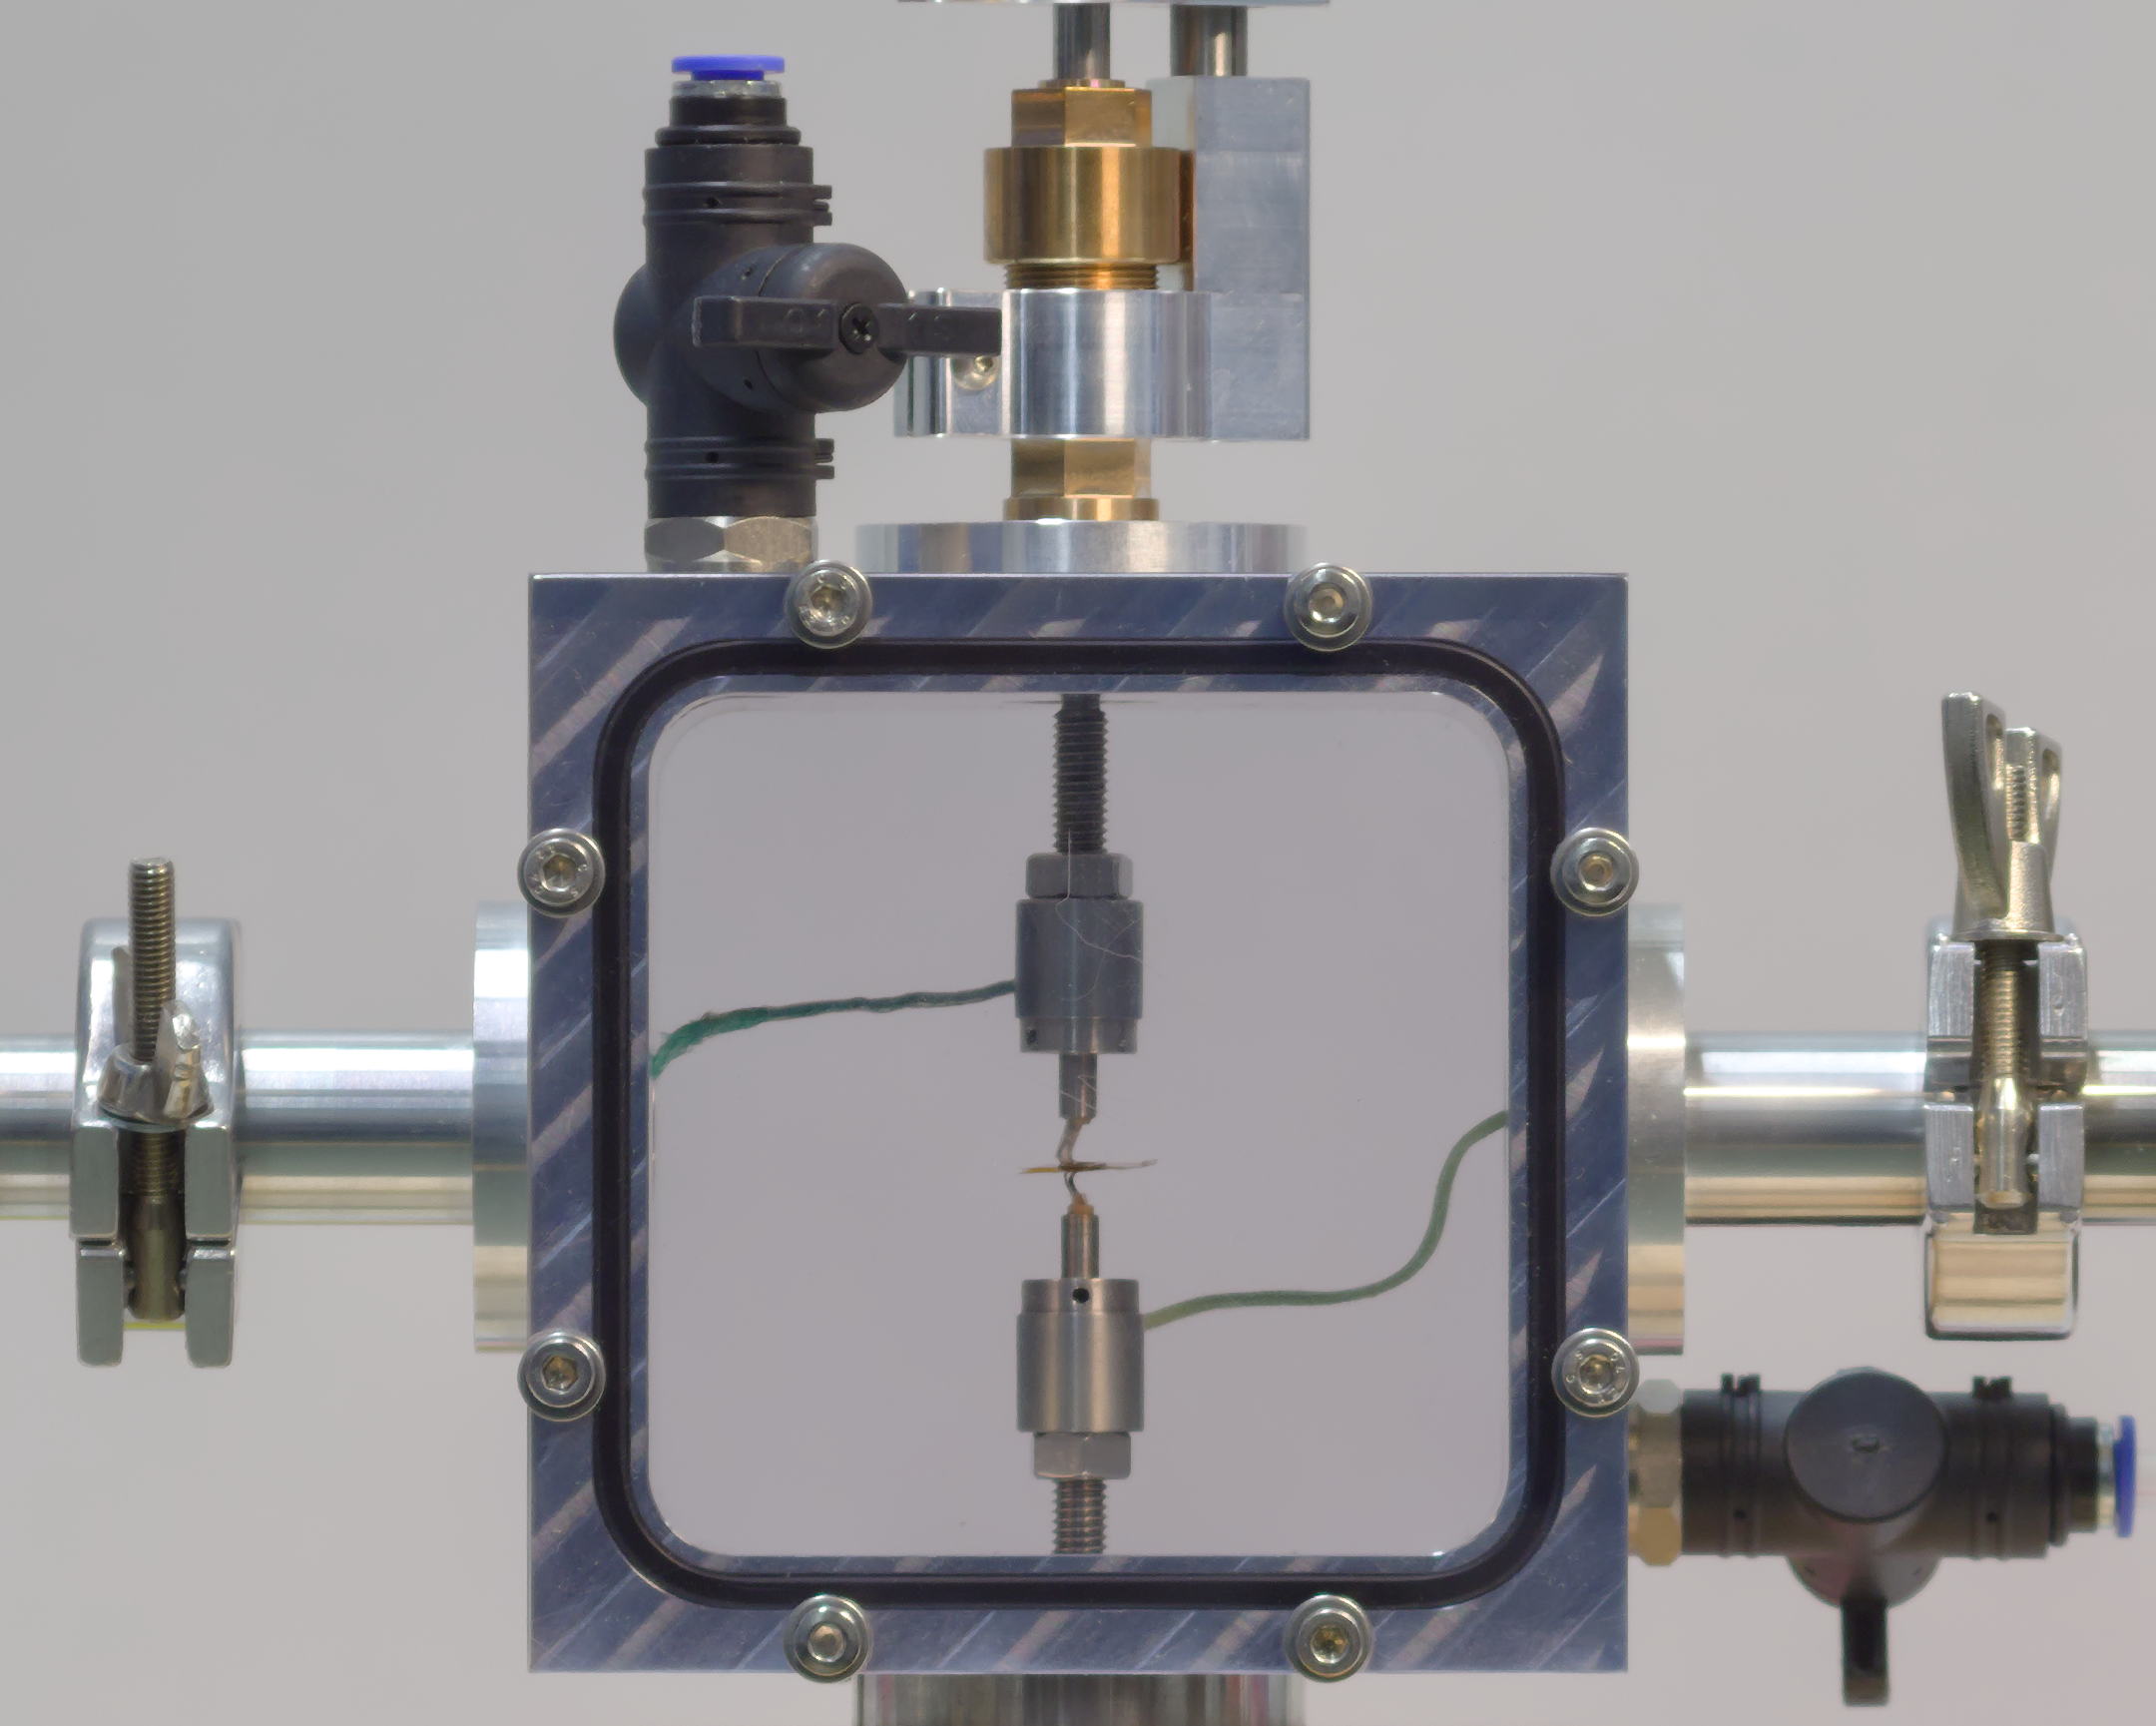
\includegraphics[width=0.8\linewidth]{bilder/gasbox_kleiner.png}
	\caption{Die Gasbox, in der das Plasma gezündet wird.}
	\label{fig:gasbox}
\end{figure}


Das Kernstück des Aufbaus ist die in Abb. \ref{fig:gasbox} abgebildete Gasbox, in der das Plasma gezündet wird. Die Box besteht aus Stahl mit zwei Fenstern zur Beobachtung und als Öffnung zum Einbau der PTPs. In dieser Box befinden sich zwei Thermosonden, die auch als Elektroden zum Zünden des Mikroplasmas dienen. Die untere Sonde ist auf ein festes Gewinde geschraubt, die obere Sonde ist senkrecht über eine Durchführung nach außen verschiebbar. Mit einer Mikrometerschraube ist die Höhe der Sonde fein einstellbar. Da die Position der Sondenplättchen auf den biegsamen Kabeln nicht vollständig fest ist, dient die Mikrometerschraube zwar zur feinen Einstellung, eignet sich aber nicht, um die Position mehrfach und reproduzierbar gleich einzustellen. Zur Einhaltung des Elektrodenabstandes wird daher ein dielektrischer Abstandshalter aus Kapton mit einem Loch in der Mitte als Zündraum verwendet. Die Kabel der Thermosonden werden durch Flansche zu den Ausleseplatinen geführt, die sich in T-Stücken auch in der Gasatmosphäre befinden. Dies vermeidet, die gewebeummantelten Kabel der PTPs nach außen führen zu müssen, was eine potenzielle Leckstelle wäre. Zudem gibt es noch zwei Gasanschlüsse als Ein- und Auslässe, entweder zum Durchspülen oder zum Abpumpen mit einer Vakuumpumpe. Dabei wird für Gase wie Helium, die leichter sind als Luft, das obere Ventil als Einlass genutzt, um die Luft in der Kammer nach unten durch das zweite Ventil zu verdrängen. Für dichtere Gase würden die Eingänge vertauscht. Über ein Manometer am Auslass lässt sich der Druck im Inneren der Kammer messen. Dieser Aufbau ist eine speziell auf PTP Messungen ausgelegte Weiterentwicklung der Gasbox aus \cite{hansenConventionalNonconventionalDiagnostics2022}, da mit geringerem Gasvolumen und ohne konstantes Spülen gearbeitet werden kann.


\section{Elektrischer Schaltplan}

\begin{figure}[h]
	\centering
	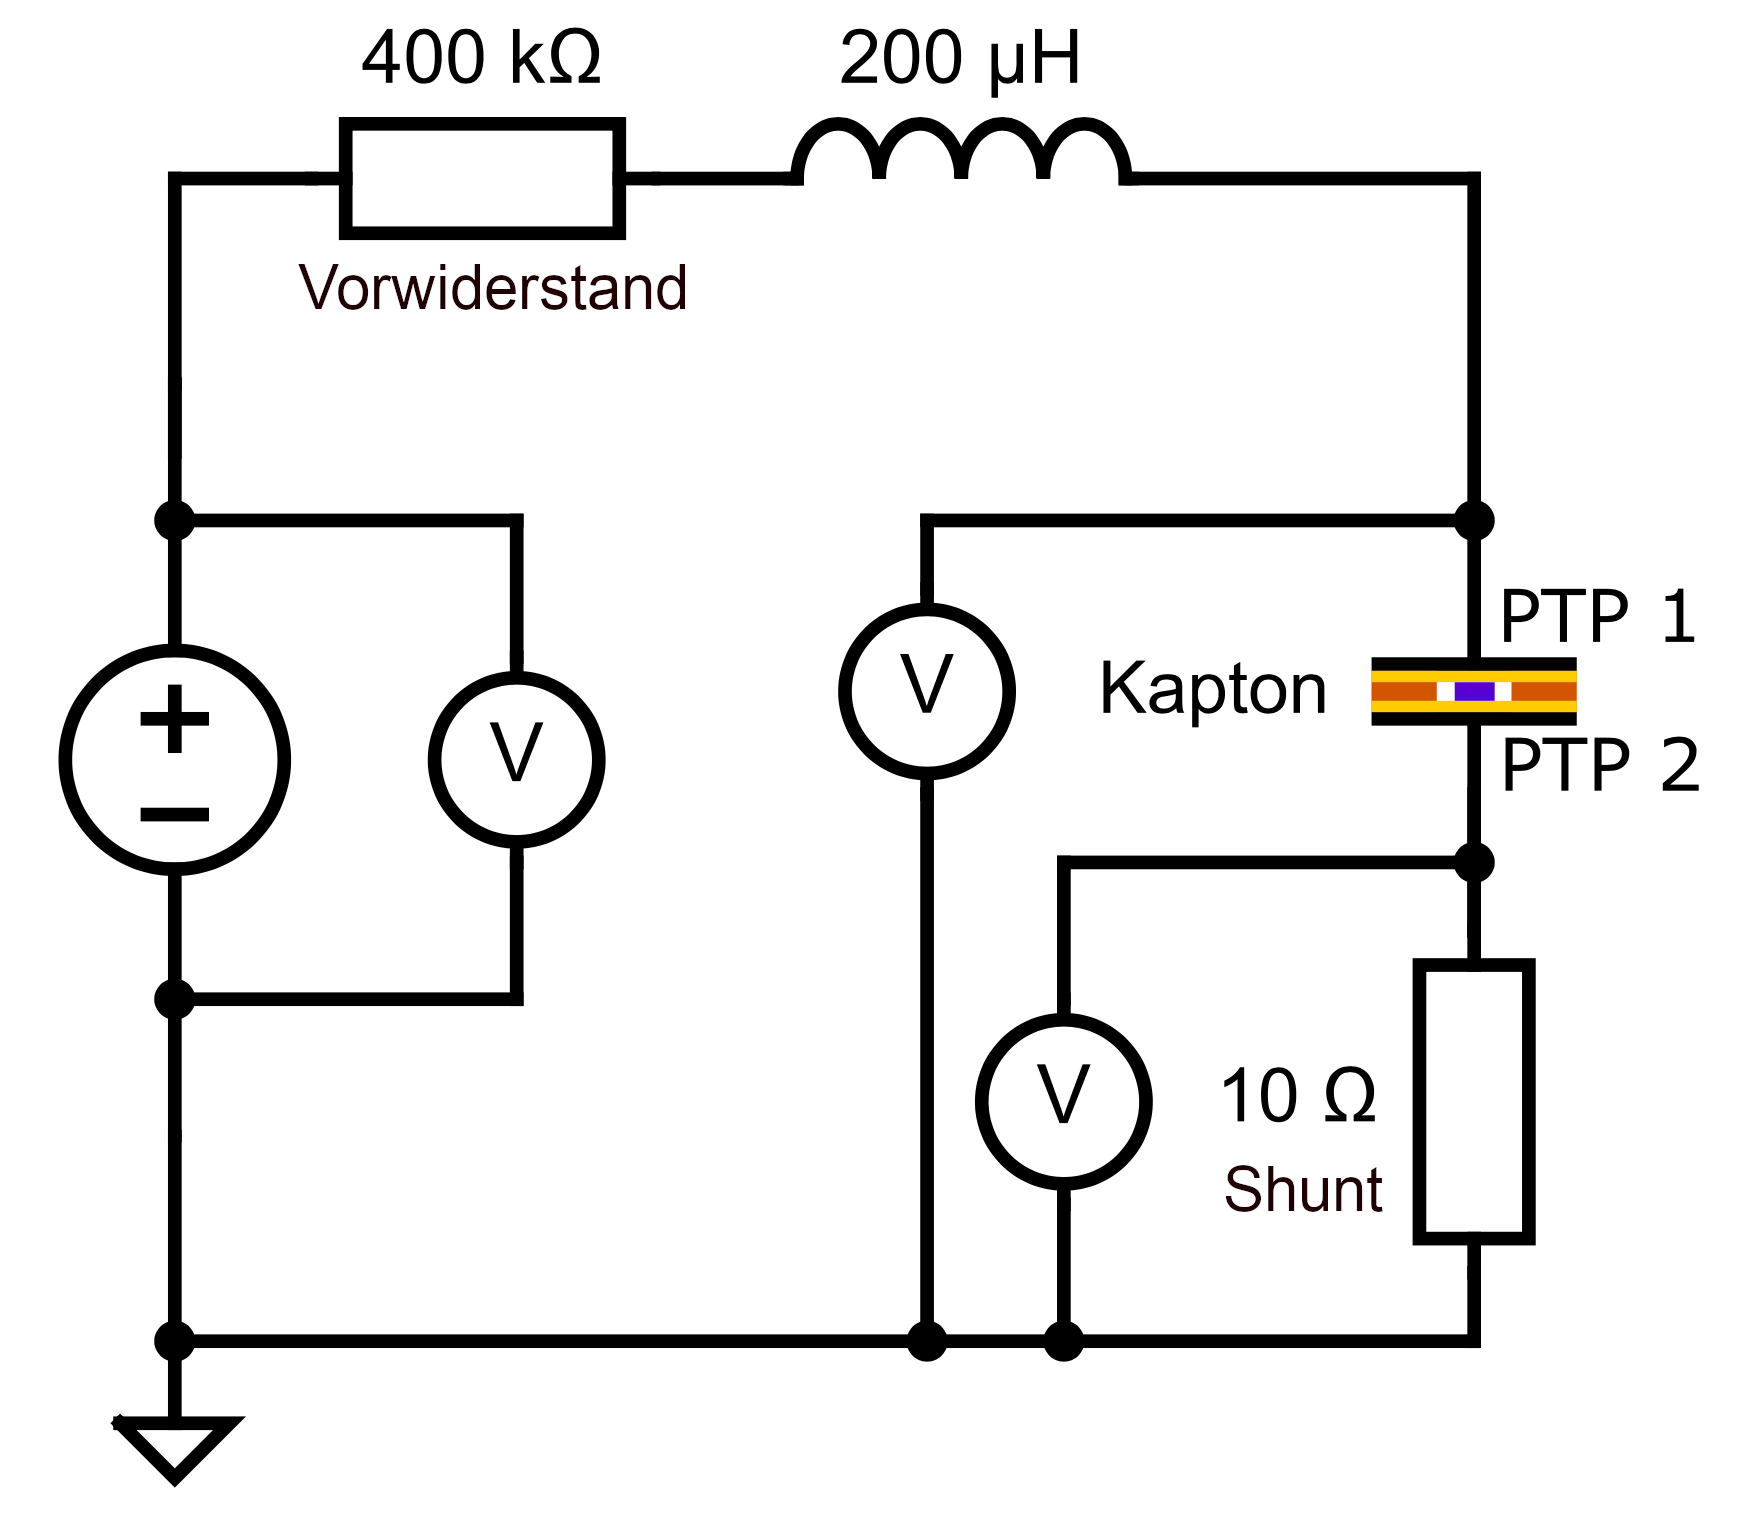
\includegraphics[width=0.5\linewidth]{bilder/schaltbild_beschriftet.png}
	\caption{Schaltbild des elektrischen Schaltkreises der Mikroplasmakammer. Als Elektroden dienen zwei PTPs. Hochspannungsmessköpfe messen die Spannungen am Netzteil, dem Mikroplasma und über dem Shunt-Widerstand. Bild aus \cite{hansenConventionalNonconventionalDiagnostics2022}.}
	\label{fig:schaltbild}
\end{figure}


Aus der Gasbox werden je PTP zweierlei Kabel herausgeführt. Zum einen werden über eine RS232-Verbindung die Daten der PTP-Platinen ausgelesen. Diese werden über einen galvanisch getrennten USB auf Seriell-Wandler (Delock 62502) an die Auswertungsrechner angeschlossen, was die Messung deutlich robuster gegenüber Stromstößen durch Arcing macht. Zudem wird über eine SHV-Stecker-Durchführung die elektrische Verbindung zum Plasma hergestellt. Der Schaltkreis für den Betrieb des Plasmas wird in Abb. \ref{fig:schaltbild} gezeigt. Von der Spannungsquelle (Heinzinger PNC 3500-300 ump) kommend, fließt der Strom zunächst durch eine Induktivität von \qty{200}{\micro\henry} und einen Vorwiderstand von \qty{400}{\kilo\ohm}. Danach wird er durch die Durchführung in die Gasbox geführt, wo das Plasma als Verbindung dient. Durch die zweite Durchführung wird der Strom nach außen und anschließend durch einen Shunt in die Erde geführt. Die elektronischen Daten werden mit drei Oszilloskoptastköpfen aufgenommen. Ein 1:1000 Tastkopf (Tektronix P6015A) misst zwischen Hochspannungseingang und Erde die gesamte von der Spannungsquelle ausgegebene Spannung. Ein 1:100 Tastkopf (Tektronix P5100A) wird nach dem Vorwiderstand angelegt und misst die über dem Plasma abfallende Spannung. Ein 1:1 Tastkopf (Tektronix P2200) misst schließlich über den Shunt den durch das Plasma fließenden Strom. Die von den Tastköpfen gemessenen Daten werden über ein Oszilloskop\footnote{PicoScope 5442B} ausgelesen und gespeichert.

\section{Elektroden und Aufbau des Mikroplasmas}

\begin{figure}[h]
	\centering
	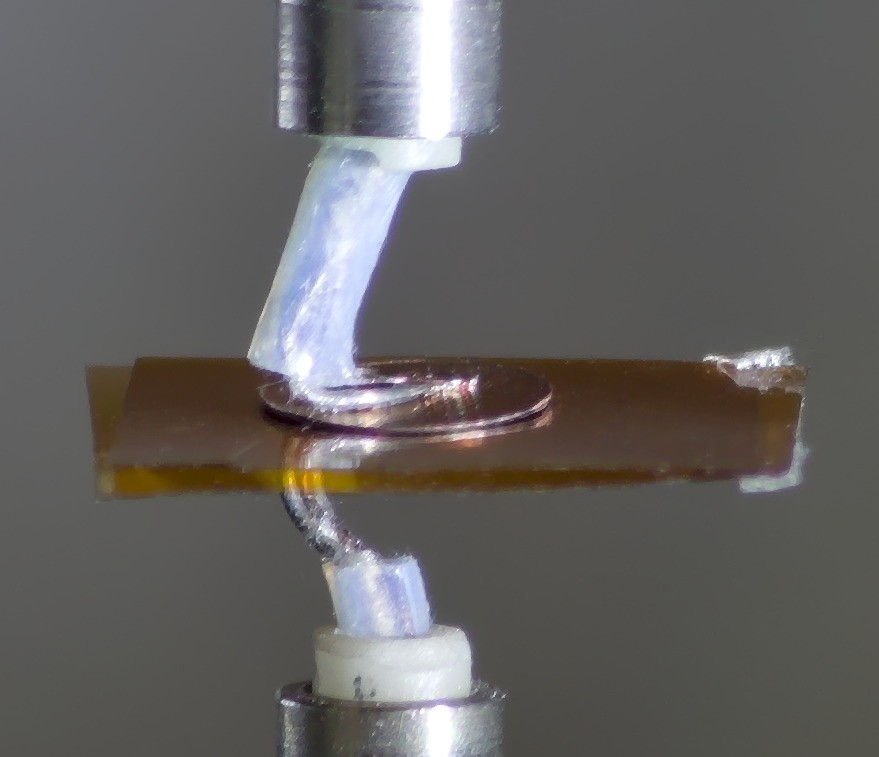
\includegraphics[width=0.7\linewidth]{bilder/plaettchenbesser.jpg}
	\caption{Nahaufnahme der eingebauten Elektroden samt Kaptonfolie.}
	\label{fig:plaettchen}
\end{figure}

Zwischen den beiden PTP-Plättchen als Elektroden wird das Mikroplasma gezündet. Um den Abstand von \qty{100}{\um} sicherzustellen, wird zwischen den Sonden eine zweilagige Kapton-Folie eingelegt, in der sich ein Loch von 1mm Durchmesser befindet. Auf diese Folie werden mit leichtem Druck die Sonden angedrückt, was sowohl die Folie glättet, als auch die Sondenplättchen parallel zueinander ausrichtet, da diese an den etwas biegsamen Verbindungsdrähten befestigt sind. Kapton wird als dielektrischer Abstandshalter benutzt, da es hitzebeständig und durchschlagfest ist und bei Unterdruck nicht ausgast. Abb. \ref{fig:plaettchen} zeigt eine Nahaufnahme dieser Elektroden.

\section{Ablauf der Energiestrommessungen}\label{sec:ablauf_energie}

Im Laufe der Energiestrommessungen wird für jedes Elektrodenmaterial die gleiche Messreihe durchgeführt. Dabei wird die Leistung des Plasmas auf die Elektroden für verschiedene Spannungen am Netzteil und damit für verschiedene Gesamtleistungen vermessen. Da mindestens \qty{500}{V} zur Zündung der Entladung benötigt werden (siehe \ref{sec:zuendspannung}), ist dies eine untere Grenze für den messbaren Bereich. Um ausreichend über der Zündspannung zu arbeiten und keine zu hohen Leistungen zu nutzen, wurden Werte von \qtyrange{700}{1000}{V} in \qty{50}{V} Schritten in sowohl positiver als auch negativer Polarität genutzt.

Im Laufe der Messreihe wird von \qty{700}{V} aufwärts gemessen, wobei die \qty{700}{V}-Messung zur Prüfung der Vergleichbarkeit am Ende der Reihe wiederholt wird. 
Die Messung bei einem Spannungswert besteht dabei aus sechs der in \ref{messprinzip} beschriebenen Temperaturpeaks. Bei jedem dieser Peaks ist das Mikroplasma dabei jeweils für \qty{10}{s} an- und dann für \qty{30}{s} ausgeschaltet. In \qty{10}{s} kann eine ausreichend lange Temperaturzeitreihe aufgenommen werden, um die dT-Auswertung zu benutzen und der Einfluss von zeitabhängigen Abweichungen beim Umschalten des Plasmas wird begrenzt. Gleichzeitig bleiben die äußeren Bedingungen, besonders die Außentemperatur, auf dieser Zeitskala unverändert, was eine wichtige Annahme der Auswertungsmethode rechtfertigt. In den \qty{30}{s}, für die das Plasma ausgeschaltet bleibt, ist genug Zeit, dass die Temperatur der Sonden auf weniger als \qty{0,5}{\celsius} über der Ausgangstemperatur vor der Messung absinkt. Dies gewährleistet eine Vergleichbarkeit der Messpeaks untereinander, da sich die Grundtemperatur im Laufe der Messung nicht relevant erhöht.

Die Wirkungsgrade und ESEEC werden aus der Messreihe für jede Spannung einzeln berechnet und gemittelt. Damit baut ein gemessener Sekundärelektronenkoeffizient auf den Messdaten von 42 Messpeaks auf\footnote{Bzw. 84, wenn auch über beide Polungen gemittelt wird.}, was den statistischen Fehler gering hält. Bei Kupfer wurde zusätzlich eine zweite dieser Messreihen bei vertauschten Sonden durchgeführt, um zu überprüfen, ob eine im Messprozess ggf. bewirkte Änderung der Oberflächenstruktur einen Einfluss auf die ESEEC hat. Da sich kein signifikanter Unterschied der ESEEC ergab, wurde der schlussendliche Koeffizient aus dem Mittelwert beider Messungen gebildet, womit pro Spannung und Polung effektiv 12 statt 6 Messpeaks genutzt wurden.

\section{Aufbau der optischen Emissionsspektroskopie (OES)}

Um die Gasreinheit innerhalb des Plasmas zu überprüfen, wurden optische Emissionsspektren der Entladung aufgenommen. Dafür wurde eine Glasfaser mit einer Fokussierungslinse auf die Entladung ausgerichtet, die die Strahlung dann in ein Spektroskop (OceanOptics HR2000+CG-UV-NIR) leitet. Pro Messung wurde dabei je ein Hell- und ein Dunkelspektrum aufgenommen, um systematische Fehler herauszurechnen. Da aus vorherigen Arbeiten bekannt ist, dass die Emissionsspektren während des Betriebs des Mikroplasmas konstant bleiben \cite{hansenConventionalNonconventionalDiagnostics2022}, wurde hier nur alle zehn Minuten ein Spektrum aufgenommen, um die Gasreinheit zu kontrollieren.
\chapter{Auswertung und Diskussion}

Diese Arbeit befasst sich sowohl mit der Nutzung von Energiestromdaten zur Berechnung effektiver SEEC, als auch mit der Methodik zur Aufnahme der nötigen Daten und den Verfahren, mit denen sich die für diese Messungen nötigen Rahmenbedingungen herstellen lassen. Deshalb werden auch in der Auswertung der gesammelten Daten Fragestellungen aus diesen verschiedenen Bereichen betrachtet.
Insbesondere stellen sich dabei folgende Fragen:
\begin{itemize}
	\item Wie lässt sich die nötige Gasreinheit sicherstellen?
	\item Wie kann die Gasreinheit im Laufe der Messung aufrechterhalten werden?
	\item Welche Verunreinigungen können auftreten und wie lassen sie sich vermeiden?
	\item Wie kann die Entladung auf Verunreinigungen überprüft werden?
	\item Wie kann überprüft werden, ob sich zwischen den Elektroden eine Glimmentladung ausbildet?
	\item Welche Spannung ist zur Erzeugung des Mikroplasmas notwendig?
	\item Welcher Wirkungsgrad kann in dieser Entladung erreicht werden?
	\item Welche Fehler treten in der Messung der Energieströme und ESEEC auf?
	\item Welche Leistungen und Energieströme fließen auf die Thermosonden?
	\item Was sind die ESEEC bei den vermessenen Metall-Gas-Kombinationen?
\end{itemize}

\section{Herstellung der notwendigen Rahmenbedingungen}\label{sec:gasreinheit}

Die Reinheit des Arbeitsgases ist für einen stabilen Betrieb des Plasmas von höchster Relevanz. Deshalb wurde zunächst untersucht, wie sich diese im weiteren Verlauf der Messungen zuverlässig herstellen lässt. Dazu wurden vor allem zwei aus der Literatur bekannte Methoden versucht: Ein mehrfaches Abpumpen und Wiederbefüllen der Kammer \cite{arumugamEffectiveSecondaryElectron2017} und ein Durchspülen der Kammer mit dem Arbeitsgas \cite{hansenConventionalNonconventionalDiagnostics2022}. Als Maß für das Bestehen einer hinreichenden Gasreinheit wird hier stets die Stabilität des Plasmas betrachtet, wie sie aus den elektronischen Daten erkennbar ist. Gibt es Verunreinigungen im Gas, bilden sich Instabilitäten in Form von Funken- bzw. Bogenentladungen.\footnote{Dieser Effekt wird in Abschnitt \ref{sec:probleme} ausführlicher besprochen.} Bei reinerer Gasatmosphäre werden diese seltener, bis sie schließlich ganz verschwinden. Dieser Zustand wird bei allen Messungen angestrebt.
\paragraph{Durchspülen der Kammer:}
Zuerst wurde der Gasschlauch für eine Minute mit einem Gasfluss von 2 slm durchgespült. Dies soll sicherstellen, dass Verunreinigungen, die in den zuvor offenen Schlauch eindringen konnten, aus diesem entfernt werden. Mit der gleichen Rate wird die Kammer nun 15 Minuten lang gefüllt, wobei das Auslassventil offen bleibt. Im Anschluss wird die Flussrate auf $ 0,\!5 $ slm eingestellt und das Auslassventil teilweise geschlossen. So wird die Kammer gespült, ohne dass Luft durch den Auslass eindringt. Regelmäßig wurde überprüft, ob eine hinreichende Gasreinheit erlangt wurde. Nach etwa 2 Stunden konnte ein stabiles Plasma gezündet werden. Das Spülen dauert so lange, da das Gas nur schwer durch den engen Zwischenraum zwischen Kapton-Folie und Elektrode hindurch diffundiert. 
\paragraph{Abpumpen und Befüllen der Kammer:}
Da die Gasbox dafür ausgelegt ist, ein Grobvakuum halten zu können, liegt es nahe, die Luft vor dem Befüllen mit Gas aus der Kammer herauszupumpen. Dabei kann die Kammer auf \qtyrange{0.1}{0.05}{\bar} abgepumpt und mit reinem Gas befüllt werden. Wird dieser Prozess fünffach wiederholt, reicht dies für ein zuverlässiges Zünden des Plasmas aus. In der Praxis hat es sich als hilfreich herausgestellt, die Kammer bei der letzten Befüllung auf leichten Überdruck zu bringen, der dann beim Verschließen der Ventile abgelassen wird. Dies verhindert eine Kontamination mit der Außenluft nach der Befüllung.


Im Vergleich der beiden Prozesse ist das zweite Verfahren schneller und zuverlässiger. Zudem werden im Spülprozess innerhalb von 2 Stunden etwa \qty{60}{\litre} Gas verbraucht, während beim Abpumpen bloß \qtyrange{1}{1,5}{\litre} pro Wiederholung verbraucht werden. Besonders bei Helium ist der geringere Verbrauch wichtig. Aus diesen Gründen wird im weiteren Verlauf der Messungen das Verfahren, fünffach abzupumpen und zu befüllen, zur Vorbereitung der Messung genutzt.

\paragraph{Erhaltung der Gasreinheit während der Messung:}
Wird zu Beginn der Messung eine reine Gasatmosphäre hergestellt und die Box verschlossen, bleibt diese Reinheit erhalten. Durch die sorgfältige Abdichtung der Eingänge durch O-Ringe gibt es nur sehr wenig Austausch von Gas mit der Umgebung. Erst über einen Zeitraum von mehreren Stunden ließ sich eine langsame Verunreinigung bemerken. In mehreren Versuchen war eine Zündung des Plasmas nach über 48 Stunden noch möglich, auch wenn das Plasma dabei instabiler war. Da eine Messreihe nur über einen Zeitraum von 2-3 Stunden geht, reicht eine Befüllung nach obigem Verfahren am Anfang aus und es gibt keinen laufenden Gasverbrauch während der Messung.

\paragraph{Weitere Verunreinigungen:} Neben mangelhafter Reinheit beim Füllen der Gasbox zeigten sich noch weitere Gründe für Instabilitäten. Am Anfang einer Messreihe kommt es oft zu unkontrollierten Bogenentladungen, welche nach einigen Versuchen abklingen. Dies kann durch Oxidschichten verursacht werden, die sich bei der Lagerung an der Luft auf den Sondenplättchen bilden. Die anfänglichen Bogenentladungen entfernen diese Oxidschichten, sodass danach eine stabile Entladung möglich ist. Zur Reinigung der Plättchen und des Abstandhalters können diese vor der Messung mit Isopropanol abgewischt werden, um Verunreinigung durch Staub zu vermeiden. Auch das Innere der Box kann so gereinigt werden, dies hatte jedoch keinen merklichen Einfluss auf die Reinheit, da die Kapton-Folie verhindert, dass Staubteilchen von außen das Plasma verunreinigen.

\subsection{Optische Emissionsspektroskopie}

Das Emissionsspektrum des Mikroplasmas zeigt ein Linienspektrum der angeregten Atome. Die genauere Untersuchung dieser Linien zeigt, dass die meisten durch angeregtes Helium erzeugt werden. Zur Identifikation der Linien wurde dabei die \textit{Atomic Spectra Database} des amerikanischen \textit{National Institute of Standards} genutzt \cite{AtomicSpectraDatabase2009}. Diese Linien treten in allen OES-Messungen am Heliumplasma auf und haben, wie in Abb. \ref{fig:spektren} sichtbar, relativ zueinander stets ähnliche Höhen. Zusätzlich ist eine prominente Sauerstoff-Linie bei ca. \qty{777}{\nm} erkennbar. Diese variiert, anders als die Heliumlinien, in ihrer Intensität relativ zu diesen und weist auf einen variablen verunreinigenden Anteil durch Sauerstoff hin. Gleichzeitig kann aus den OES-Daten gefolgert werden, dass diese Verunreinigung nicht durch ein Leck zur Außenluft erzeugt wird, da sonst ein deutliches Liniensystem des Stickstoffs um \qty{379}{\nm} erkennbar wäre. Dieses ist in Abb. \ref{fig:spektren} nicht sichtbar. Weiterhin zeigt das Fehlen der Stickstofflinien, dass beim Befüllen der Kammer keine signifikante Menge an Luft in dieser verblieben ist. Stattdessen wird diese Verunreinigung wahrscheinlich durch die Abtragung einer Oxidschicht auf der Sondenoberfläche erzeugt, die sich bei deren Lagerung an der Außenluft bildet. 

\begin{figure}[h]
	\centering
	\includesvg[width=0.9\linewidth]{plots/spektrum_vergleich}
	\caption{Zwei Spektren am Heliumplasma mit verschiedenem Elektrodenmaterial: \textbf{a)} Kupfer, \textbf{b)} Nickel}
	\label{fig:spektren}
\end{figure}

Wird im Laufe einer Messreihe an mehreren Zeitpunkten ein Spektrum aufgezeichnet, so kann der zeitliche Verlauf der relativen Linienstärken betrachtet werden. Dies wird in Abb. \ref{fig:spektralverlauf} dargestellt. Im Versuch treten keine deutlichen Änderungen im Zeitverlauf auf. Dass sich die Stärke der O I-Linie nicht verändert, impliziert wiederum, dass sie nicht durch ein dauerndes Leck der Gasbox verursacht wird, da sonst im Laufe der Messung immer mehr Sauerstoff in die Gasatmosphäre diffundieren würde.

\begin{figure}[h]
	\centering
	\includesvg[width=0.9\linewidth]{plots/heni_verlauf}
	\caption{Relative Linienstärken im Verlauf der Messung. Die Spektren wurden je in Abständen von 10 Minuten aufgenommen, wobei das Plasma für insgesamt etwa 2 Minuten gezündet wurde. Die Sauerstofflinie ist hier in schwarz abgebildet.}
	\label{fig:spektralverlauf}
\end{figure}



\section{Überprüfung der erfolgreichen Zündung einer Glimmentladung}

\paragraph{Strom-Spannungskennlinien:}

\begin{figure}[h]
	\centering
	\includesvg[width=0.9\linewidth]{plots/ui_kennlinie2}
	\caption{\textbf{a)} Strom-Spannungs-Kennlinien des Plasmas. \textbf{b,c)} Nähere Ausschnitte der Linien um die gleichbleibende Spannung zu zeigen.}
	\label{fig:kennlinien}
\end{figure}

Normale Glimmentladungen haben die Besonderheit, dass die über dem Plasma abfallende Spannung unabhängig vom fließenden Strom ist \cite{demtroederExperimentalphysik2013,franzLowPressurePlasmas2009}. Nach erfolgter Zündung führt eine Erhöhung des Stroms nur noch zu einer Ausweitung des Entladungskanals, nicht jedoch zu einer Erhöhung der Stromdichte im Kanal \cite{hansenConventionalNonconventionalDiagnostics2022}. Dies kann am Aufbau durch Messung mit dem Oszilloskop überprüft werden. Tatsächlich sind in der so erhaltenen Kennlinie, gezeigt in Abb. \ref{fig:kennlinien}, nur geringe Schwankungen sichtbar. Dabei stellen sich Spannungen von \qtyrange{150}{160}{V} bei Nickelelektroden und \qtyrange{190}{210}{V} bei Kupferelektroden ein. Die Entladung kann bis zu einem Strom von \qty{0.5}{\mA} betrieben werden, bei kleineren Strömen verlöscht das Plasma.


\paragraph{Emissionslinien im Spektrum:}

Im Spektrum der Entladung lassen sich klar die Emissionslinien des Arbeitsgases erkennen und kein Schwarzkörperanteil. Das zeigt, dass das Leuchten durch elektronische Anregung entsteht, wie es in einem Nichtgleichgewichtsplasma der Fall sein sollte.

\section{Größe der Zündspannung}\label{sec:zuendspannung}

Um die zum Zünden des Mikroplasmas mindestens nötige Spannung zu bestimmen, wurde der Zündprozess genauer betrachtet. Insbesondere wurden dabei die Datenreihen ausgewertet, in denen es vor dem Erreichen einer stabilen Glimmentladung nicht zu Funkenentladungen kam. Ein Beispiel einer Entladung mit solchen Instabilitäten zeigt Abb. \ref{fig:zuendspannung}b). Die Zeitreihen sind in Abb. \ref{fig:zuendspannung} dargestellt. Beim Erhöhen der anliegenden Spannung durch die Quelle fällt zunächst alle Spannung über den Elektroden ab, da der Zündraum ohne Plasma nicht leitfähig ist. Die Spannung wächst, bis das Plasma schließlich zündet. Nach dem Überschreiten dieser Hürde fällt die Spannung schnell auf einen vom Strom unabhängigen Wert ab. Die Zündspannung ist dann die maximal erreichte Spannung vor dem Beginn des Stromflusses. Da die Zielspannung der Spannungsquelle zum Zeitpunkt der Zündung noch nicht erreicht ist, sollte sie keinen Einfluss auf die Zündspannung haben. %Da das Zünden durch Instabilitäten erschwert oder, wie beim Arcing ganz verhindert werden kann, ist es sinnvoll, mehrere solche Messungen auszunehmen und von diesen die niedrigste Zündspannung auszuwählen. Diese ist am wenigsten durch Fehler beeinträchtigt, ermöglicht aber immernoch eine Plasmazündung.
Aus den Zeitreihen ergaben sich bei Helium und Kupfersonden Werte von \qtyrange{500}{520}{V}. Dies liegt deutlich über dem aus dem Paschen-Gesetz abgeleiteten Wert von ca. \qty{120}{V}, was in der Praxis auch zu erwarten ist.


\begin{figure}[h]
	\centering
	\includesvg[width=0.9\linewidth]{plots/zuendspannung}
	\caption{Strom-Spannungs-Verläufe zur Bestimmung der Zündspannung: \textbf{a)} zeigt eine stabile Plasmazündung bei \qty{510}{V}, \textbf{b)} eine instabilere Zündung mit einigen Funkenentladungen. Unabhängig vom Verlauf der Zündung stellen sich die gleichen konstanten Werte für Spannung und Strom ein.}
	\label{fig:zuendspannung}
\end{figure}



\section{Wirkungsgrad der Entladung}

Als Wirkungsgrad wird hier das Verhältnis der thermischen Leistung $ P_\text{therm, ges} $ an beiden Sonden zur gesamten elektrischen Leistung $ P_\text{el} $ am System betrachtet. Dies ist eine nützliche Größe, da gerade die auf die Sonden gerichtete Energie in der Praxis zur Bearbeitung einer Oberfläche zur Verfügung steht. Konvektion des heißen Gases nach außen tritt nur sehr wenig auf, da der Gasfluss durch den Spacer größtenteils verhindert wird. Da der Abstand zwischen den Elektroden im Vergleich zu deren Durchmesser klein ist, wird der Großteil der Wärmeleistung von diesen aufgenommen. Aufgrund der Geometrie ist ein hoher und von der Gesamtleistung unabhängiger Wirkungsgrad zu erwarten. Werden mehrere Messungen bei verschiedenen Gesamtleistungen angestellt, kann der Wirkungsgrad durch lineare Regression der gesamten thermischen Leistung gegen die elektrische Leistung bestimmt werden. Das Verfahren und die Ergebnisse sind in Abb. \ref{fig:wirkungsgrad} dargestellt. Dabei ergaben sich die in Tab. \ref{tab:eta} notierten Werte.

\begin{table}[thb]
	\centering
	\begin{tabular}{ccr}
		
		{Material} &{$ \eta $} \\
		\toprule
		
		{Kupfer}      & \num{86(3)}\%  \\
		%\midrule
		{Tantal}      & \num{85(4)}\%   \\
		%\midrule
		{Edelstahl}      & \num{97(4)}\%   \\
		%\midrule
		\addlinespace
		
	\end{tabular}
	
	\caption{Werte der Wirkungsgrade im Heliumplasma.}
	\label{tab:eta}
\end{table}

\begin{figure}[h]
	\centering
	\includesvg[width=0.9\linewidth]{plots/wirkungsgrad}
	\caption{\textbf{a)} Bestimmung des Wirkungsgrades der Entladungen bei verschiedenen Sondenmaterialien durch lineare Regression auf den Leistungsmesspunkten. \textbf{b)} Berechnete Wirkungsgrade.}
	\label{fig:wirkungsgrad}
\end{figure}


\section{Betrachtung der Fehler in der Messung der ESEEC}

Die Ungenauigkeit bei der Bestimmung der ESEEC setzt sich aus Fehlern zweier Art zusammen: Zum einen treten bei der Messung Schwankungen der elektrischen und thermischen Leistungswerte auf. Aus diesen ergibt sich ein statistischer Fehler über die Standardabweichung der Messwerte. Des weiteren gibt es aber auch für jede Sonde eine Ungenauigkeit bei der Bestimmung der Wärmekapazität. Da diese kein fluktuierender Effekt ist, sondern sich als gleichbleibende Abweichung des bekannten zum wahren Wert der Wärmekapazität zeigt, lässt sie sich nicht durch wiederholte Messreihen an der gleichen Sonde verbessern.


Im Prozess der Kalibrierung kann es zu verschiedenen Fehlern kommen. Zunächst ergibt sich in der Kalibrierungsauswertung ein Fehler von etwa 2-3\% aus der Statistik der Einzelmessungen während der Kalibrierung. Da die Wärmekapazität der Sonde ein Effektivwert ist, der auch die Ableitung von Wärme über den Sondendraht beschreibt, ist sie nicht gänzlich unabhängig von der Art und Weise der Erhitzung. Die Menge an Wärme, die weggeleitet wird, ist dabei abhängig vom Temperaturgradienten im Draht. Würde die Sonde also auf eine deutlich höhere Temperatur erhitzt als bei der Kalibrierung, wären die Kalibrierungsdaten nur eingeschränkt nutzbar. In diesem Experiment wird die Sonde dagegen nur auf etwa \qty{70}{\celsius} erhitzt, was gut vergleichbar mit den Temperaturen beim Kalibrieren ist.


Die in der dT-Auswertung berechnete Leistung ergibt sich aus der Änderung der Sondentemperatur\footnote{Bzw. dem Anteil, der durch die Heizleistung verursacht wird, hier auch $ \dot{T} $ genannt.} und der Wärmekapazität der Sonde. 
\begin{align*}
	P = C\dot{T}
\end{align*}

Dementsprechend ist der relative Fehler der Leistung gerade die Summe aus dem relativen statistischen Fehler der Temperaturänderungen und dem relativen Fehler der Wärmekapazität. Der Einfachheit halber wird dieser immer als 3\% angenommen, was leicht über dem üblichen Wert liegt.
\begin{align*}
 \dfrac{\Delta P}{P} = \dfrac{\Delta \dot{T}}{ \dot{T}} + \dfrac{\Delta C}{C}
\end{align*}

Auch die Fehler der ESEEC teilen sich in der Rechnung in statistische Schwankungen und fehlerhafte Wärmekapazitäten auf:
\begin{align*}
	\gamma_\text{E} &= \dfrac{P_\text{el}}{P_\text{therm,C}}\\
	\Delta \gamma_\text{E} &= \dfrac{1}{P_\text{el}} \Delta P_\text{el} + \dfrac{P_\text{el}}{P_\text{therm,C}^2} \Delta P_\text{therm,C}\\
					&= \dfrac{P_\text{el}}{P_\text{therm,C}} \left( \dfrac{\Delta P_\text{el}}{P_\text{el}} + \dfrac{\Delta P_\text{therm,C}}{P_\text{therm,C}} \right)\\
					&= \dfrac{P_\text{el}}{P_\text{therm,C}} \left( \underbrace{\dfrac{\Delta P_\text{el}}{P_\text{el}} + \dfrac{\Delta \dot{T}}{ \dot{T}}}_{\text{statistische Fehler}} + \underbrace{\dfrac{\Delta C}{C}}_\text{systematischer Fehler} \right)
\end{align*}

%Da die Sonden bei der Kalibration standardmäßig für 30 s geheizt werden, in meinen Versuchen aber nur für 10 s am Stück mit deutlich höherer Leistung, lassen sich die effektiven Wärmekapazitäten auch nur eingeschränkt verwenden. Besonders bei den hier verwendeten kleinen Sondenplättchen mit geringer Wärmekapazität hat die thermische Trägheit durch den Rest der Sonde aber einen großen Einfluss, was diese Methode fehleranfällig macht. 



\section{Größe der Leistungen und Energieströme im Plasma}\label{sec:energiestroeme}
Die Verwendung von PTPs als Elektroden dient der direkten Messungen der Leistung aus dem Plasma. Dabei wird der Energiestrom nach der Art der Elektrode (positiv, negativ und geerdet, bzw. Kathode und Anode) aufgeteilt. Zudem wird die elektrische Leistung gemessen.\\

Üblicherweise werden die Messwerte von PTP-Messungen als Energieströme angegeben. Dies liegt daran, dass eine Niederdruckentladung deutlich größer ist, als das Plättchen der Thermosonde. Dieses fängt so nur einen kleinen Teil der Energie aus dem Plasma auf. Deshalb ist es sinnvoll, die gemessene Leistung auf die bekannte Fläche des Plättchens zu normieren. Bei Atmosphärendruckplasmen, insbesondere bei Mikroentladungen, ist das Plättchen jedoch deutlich größer als die Entladung. Im hier untersuchten Aufbau wird sogar die fast vollständige Leistung des Mikroplasmas von den Sonden aufgenommen. Deshalb ist es sinnvoller, die gemessene Leistung direkt anzugeben. Zur Berechnung der ESEEC ist zudem nur die gesamte Leistung an der Kathode und nicht der Energiestrom relevant. Um sinnvolle flächennormierte Energieströme zu berechnen, müsste man zudem die tatsächliche Fläche der Entladung messen, da nur über diese Fläche Energie auf die Sonde trifft. Eine solcher Schätzwert wird später in diesem Abschnitt berechnet.
\begin{figure}[h]
	\centering
	\includesvg[width=0.8\linewidth]{plots/energiestrom800}
	\caption{Der Energiestrom auf beide Elektroden bei verschiedenen Materialien und der gleichen Spannung.}
	\label{fig:energiestrom}
\end{figure}

Misst man für eine gegebene Spannung die thermische Leistung an beiden Elektroden, fällt auf, dass die Leistung an der Anode stets niedriger ist als die an der Kathode, was in Abb. \ref{fig:energiestrom} gut erkennbar ist. Dies liegt an der Energie der beschleunigten Ionen und durch diese zur Kathode gestoßenen Neutralteilchen \cite{hansenConventionalNonconventionalDiagnostics2022}, welche schließlich auch zur Sekundärelektronenemission beiträgt.

Die Verhältnisse zwischen den Leistungen an Kathode und Anode bleiben bei verschiedenen Leistungen ähnlich (siehe Abb. \ref{fig:einzelleistungen}), nur deren absoluter Wert ändert sich.

\begin{figure}[H]
	\centering
	\includesvg[width=0.9\linewidth]{plots/einzelleistungenKupfer}
	\caption{Der Energiestrom auf die Kupferelektroden in Helium bei verschiedenen Leistungen im Plasma.}
	\label{fig:einzelleistungen}
\end{figure}

Trotz der geringen Gesamtleistung ist die Energieflussdichte in der Entladung sehr hoch, da die Fläche der Entladung klein ist. Zum Beispiel ergibt sich mit in einem vergleichbaren Messaufbau bestimmten Querschnittsflächen von \qty{0,1}{\square\mm} in Helium bei \qty{1,5}{\mA} \cite{hansenConventionalNonconventionalDiagnostics2022} und dem hier bestimmten Leistungsübertrag auf die Kathode von \qty{0,14}{W} bei gleichem Strom ein Energie\-strom von \qty{140}{W.cm^{-2}}. Dies entspricht in etwa dem zehnfachen Energiestrom an der Spitze einer Kerzenflamme \cite{haminsCharacterizationCandleFlames2005}.
%Dies entspricht der Wärmestrahlungsdichte eines schwarzen Körpers mit ca. 2230K. Da die Wärmeleitung vom Plasma an die Elektroden über schnelle Teilchen aber deutlich effektive ist als die über Schwarzkörperstrahlung, ist die Temperatur des Plasmas aber deutlich niedriger.\footnote{Die Gleichgewichtstemperatur der Elektroden ist selten über $ 1ßß^\circ\text{C} $.} 
Die Dichte der gesamten, durch das Mikroplasma geleiteten, elektrischen Leistung erreicht bei dieser Entladung sogar ca. \qty{31}{W.mm^{-3}}. Der Energiestrom auf die Sonden ist dabei linear von der Spannung am Netzteil abhängig. Da bei einer Erhöhung der Gesamtleistung die Fläche des Entladungskanals vergrößert wird, sind diese Werte mehr oder weniger konstant. Gleiches gilt auch für die elektrische Stromdichte im Plasma \cite{hansenConventionalNonconventionalDiagnostics2022}.

\subsection{Probleme bei der Durchführung der Messreihen}\label{sec:probleme}
\paragraph{Funken- und Bogenentladungen: }
Wie schon in Abschnitt \ref{sec:gasreinheit} beschrieben wurde, ist das größte Problem für die Durchführung einer Messreihe die Bildung von Funkenentladungen anstatt eines Betriebs im Glimmbereich. Da wegen der Strombegrenzung des Netzteils nicht der nötige Strom zur Erhaltung eines Lichtbogens fließen kann, zerfällt dieser Funken schnell wieder und bildet sich erneut. Dieses Flackern ist in Abb. \ref{fig:zuendspannung} gut erkennbar. Solche Bogenentladungen könne eine Zündung des Plasmas auch ganz verhindern. 

\begin{figure}[h]
	\centering
	\includesvg[width=0.9\linewidth]{plots/arcing}
	\caption{Zeitverlauf von \textbf{(a)} Spannung und \textbf{(b)} Strom im Falle unkontrollierter Entladungen.}
	\label{fig:arcing}
\end{figure}

In der Kennlinie des Oszilloskops, ein Beispiel ist in Abb. \ref{fig:arcing} gezeigt, ist dies klar erkennbar, besonders im Vergleich zum Verlauf nach der Zündung in Abb. \ref{fig:zuendspannung}. Dieses Problem wurde in den in Teil \ref{sec:energiestroeme} ausgewerteten Messreihen durch eine saubere Befüllung gelöst wurde. Obwohl der gleiche Befüllungsprozess verwendet wurde, wurden Messungen an anderen Materialien, durch solche Instabilitäten ganz verhindert. Dies betrifft insbesondere die Messung an Aluminium, sowie alle Versuche von Messungen mit Argon als Arbeitsgas. Auch eine Veränderung des Vorwiderstandes war nicht erfolgreich.

\paragraph{Abtragung der Beschichtungen }
Die Beschichtungen der Sonden, die nicht vollständig aus dem jeweiligen Material bestehen, sind sehr empfindlich. Besonders die TiN-Schicht wird vom Plasma schnell abgetragen, da sie nur maximal \qty{150}{\nm} dick ist. Dies wurde im Verlauf der Messung an den elektrischen Daten sichtbar. Je nach Material der Sonde fallen nach dem Zünden verschiedene Spannungen über dem Plasma ab. So ist z.B. in Abb. \ref{fig:kennlinien} ein klarer Unterschied zwischen Kupfer und Nickel erkennbar. 

\begin{figure}[H]
	\centering
	\includesvg[width=0.9\linewidth]{plots/TiN_spannung}
	\caption{Über dem Plasma abfallende Spannungen verändern sich im Verlauf der Messreihe an TiN. Jede angeschriebene Spannung ist der Mittelwert von insgesamt \qty{60}{s} Betriebszeit. Umpolen der Sonden bei Messpunkt 9.}
	\label{fig:TiN_spannung}
\end{figure}

In Abb. \ref{fig:TiN_spannung} ist gut erkennbar, wie sich die abfallende Spannung während der Messreihe an TiN von einem Wert von etwa \qty{170}{V} aus den bei Kupfer üblichen Werten von \qtyrange{190}{200}{V} nähert. Das legt nahe, dass die TiN-Schicht abgetragen im Laufe der Messungen wird, bis nur noch Kupfer üblich ist. Da die einzelnen Messpunkte in Abb. \ref{fig:TiN_spannung} jeweils der Durchschnitt aus einer Minute Betriebszeit\footnote{6 Peaks a \qty{10}{s}} sind, geschieht die Abtragung der Schicht effektiv auf einer Zeitskala von wenigen Minuten. Rechnerisch ergibt sich damit eine Abtragungsrate von \qty{0,17}{\nm\per\second}. Diese ist aber nur begrenzt aussagekräftig, da die Abtragung nicht gleichmäßig geschieht. Das Loch in der Schicht konnte bei der Überprüfung der Son\-den\-ober\-flä\-chen bestätigt werden. Unkontrollierte Entladungen zwischen den Elektroden können auch dickere Beschichtungen zerstören. Nach den Zündversuchen an Aluminium-Sonden war beispielsweise die Beschichtung im Zündbereich nahezu vollständig entfernt.
 
 \paragraph{Fehler bei der Kalibrierung der Sonden }
 Auch wenn sich die statistischen Fehler der Kalibrierung zu 2\% bis 3\% ergeben, kann es manchmal zu größeren Fehlern kommen. Bei Betrachtung der gemessenen Wärmekapazitäten ist es jedoch schwierig, die Fehler der Kalibrierung von der Schwankung der wahren Werte untereinander zu unterscheiden. Ein Beispiel für einen potenziellen größeren Kalibrierungsfehler ist die Messung an den TiN-Sonden. 
 
 \begin{figure}[H]
 	\centering
 	\includesvg[width=0.9\linewidth]{plots/einzelleistungenTiN}
 	\caption{Der Energiestrom auf die TiN-Elektroden in Helium bei verschiedenen Leistungen im Plasma. Die Verhältnisse der Leistungen an den Elektroden zueinander weichen von den üblichen Werten (siehe Abb. \ref{sec:energiestroeme}) ab.}
 	\label{fig:einzelleistungenTiN}
 \end{figure}

Die an TiN gemessenen Leistungen sind in Abb. \ref{fig:einzelleistungenTiN} abgebildet und sichtbar anders als bei den anderen Metallen. Insbesondere fällt auf, dass – anders als bei allen anderen Messungen – die Kathode bei der negativ gepolten Messung weniger Leistung misst als die Anode. In der positiv gepolten Messung ist die übliche Differenz dagegen sehr stark ausgeprägt. Besonders im Vergleich mit der schwächer ausgeprägten Differenz bei Kupfer ist dies überraschend, da Abb. \ref{fig:TiN_spannung} nahelegt, dass die Elektrodenoberflächen in dieser Messung vor allem aus Kupfer bestanden. Beide Besonderheiten könnten dadurch erklärt werden, dass die vorgespannte Elektrode (in Abb. \ref{fig:TiN_spannung} in Blau bzw. Orange gekennzeichnet), die in beiden Fällen durch die selbe PTP gebildet wird, die gemessene Leistung wegen eines Kalibrierungsfehlers systematisch unterschätzt. Tatsächlich hat diese Sonde laut Kalibrierung eine Wärmekapazität von nur \qty{0,0089}{J.K^{-1}}, was deutlich unter den üblichen Werten von \qtyrange{1,1}{1,2}{J.K^{-1}} bei baugleichen PTPs liegt. Wäre die tatsächliche Wärmekapazität dieser Sonde höher und im Rahmen der anderen Sonden, ergäben sich rechnerisch mit anderen Messungen vergleichbare Ergebnisse. Aus den ersten Messungen der TiN-Sonde, bei denen die Schicht noch intakt war, ergibt sich ein ESEEC von \num{1,6}. Dieser ist aber wegen des wahrscheinlichen Kalibrierungsfehlers nicht aussagekräftig. 

\section{Bestimmung  der effektiven Sekundärelektronenemissionskoeffizienten.}

Aus den Leistungen an den jeweiligen Elektroden können nun die ESEEC bestimmt werden. Dabei ergeben sich in allen Fällen Werte von \numrange{0,7}{1,2}, die in Tab. \ref{tab:ESEEC} zusammengefasst werden. Diese sind vergleichbar mit anderen bei Atmosphärendruck bestimmten ESEEC \cite{hansenConventionalNonconventionalDiagnostics2022}. 

\begin{table}[thb]
	\centering
	\begin{tabular}{ccr|ccc}
		
		{Material} &{$ \gamma_\text{E} $}& \multicolumn{1}{l}{$ \Delta\gamma_\text{E} $} & {$ \gamma_\text{E, Niederdruck} $} & {Notiz zu Niederdruckwert} & {Quelle} \\
		\toprule
		
		{Kupfer}      & \num{1,16(6)} & 5\% & \num{0,28(5)} & gemessen an He & \cite{guntherschulzeElektronenablosungDurchStoss1930}  \\
		%\midrule
		{Tantal}      & \num{0,77(9)} & 11\% & \num{0,117} & gemessen an Ar & \cite{oechsnerElectronYieldsClean1978} \\
		%\midrule
		{Edelstahl}      & \num{0,96(8)} & 8\% & \num{0,066(10)} & gemessen an Ar & \cite{dakshaComputationallyAssistedSpectroscopic2016}  \\
		%\midrule
		\addlinespace
		
	\end{tabular}
	
	\caption{Werte der ESEEC am Heliumplasma.}
	\label{tab:ESEEC}
\end{table}

Wie erwartet sind die Werte bei Normaldruck jeweils deutlich höher als die entsprechenden Werte bei Niederdruck, die typischerweise bei etwa \numrange{0,1}{0,3} liegen und insbesondere die Werte des rein ionenbasierten SEE Koeffizienten von etwa \numrange{0,01}{0,1}  \cite{liebermanPrinciplesPlasmaDischarges2005,haaseDynamicDeterminationSecondary2018,bohmRetardingfieldAnalyzerMeasurements1993,toliasSecondaryElectronEmission2014, marcakNoteIoninducedSecondary2015,dakshaComputationallyAssistedSpectroscopic2016,pamperinIoninducedSecondaryElectron2018,dakshaMaterialDependentModeling2019,oechsnerElectronYieldsClean1978,guntherschulzeElektronenablosungDurchStoss1930}. Beispiele für diese stehen auf der rechten Seite von Tab. \ref{tab:ESEEC}, können aber nur als Anhaltspunkte genommen werden, da sie bei verschiedenen Drücken und teilweise anderen Gasen gemessen wurden.

\begin{figure}[h]
	\centering
	\includesvg[width=0.9\linewidth]{plots/eseec}
	\caption{Die effektiven SEEC der verschiedenen Materialien bei Helium, aufgeteilt nach der Polarität der Messung.}
	\label{fig:eseec}
\end{figure}

In Abb. \ref{fig:eseec} ist keine signifikante Abhängigkeit der ESEEC von der Polarität der Entladung erkennbar. Daher ist es sinnvoll, die Werte der verschiedenen Polaritäten pro Material zu einem Wert zusammenzufassen.

\paragraph{Messung an Kupfer in zwei Messreihen }
Wie in \ref{sec:ablauf_energie} beschrieben, wurden an den Kupfersonden zwei Messreihen durchgeführt, um eine Veränderung der ESEEC, die empfindlich von der Oberflächenstruktur abhängen \cite{phelpsColdcathodeDischargesBreakdown1999}, zu überprüfen. Dabei ergaben sich die in Tab. \ref{tab:ESEEC_Cu} notierten Werte.


\begin{table}[thb]
	\centering
	\begin{tabular}{ccr}
	
	{Material} &{$ \gamma_\text{E} $}& \multicolumn{1}{l}{$ \Delta\gamma_\text{E} $} \\
	\toprule
	
	{Kupfer früh}      & \num{1,16(20)} & 17\%  \\
	%\midrule
	{Kupfer spät}      & \num{1,15(11)} & 10\%  \\
	%\midrule
	{Kupfer}      & \num{1,16(6)} & 5\%  \\
	%\midrule
	\addlinespace
	
	\end{tabular}

	\caption{Werte der ESEEC am Heliumplasma.}
	\label{tab:ESEEC_Cu}
\end{table}
Dabei gibt es keinen signifikanten Unterschied zwischen der frühen und der späten Messreihe, weshalb aus diesen der schon oben genannte Mittelwert berechnet wurde. Der geringere Fehler des Mittelwertes resultiert aus der höheren Zahl an Einzelmessungen.

\chapter{Fazit und Ausblick}

In dieser Arbeit wurde die Sekundärelektronenemission an einer Mikroentladung und durch Energiestrommessungen untersucht. Insbesondere wurden die effektiven SEE Koeffizienten eines Atmosphärendruck-DC-Mikroplasmas in Helium auf verschiedenen Oberflächen bestimmt. 

Um an einem Mikroplasma Energiestrommessungen durchzuführen, wurde dieses zwischen zwei passiven Thermosonden gezündet, die als Elektroden dienten. Dafür wurden Thermosonden aus verschiedenen Materialien hergestellt und kalibriert. Es konnte gezeigt werden, das dies eine gute Methode ist, mit der nahezu der vollständige Energiestrom aus dem Plasma vermessen und auf Kathode und Anode aufgeteilt werden kann.\\

Es konnte gezeigt werden, dass die effektiven SEE Koeffizienten bei Atmosphärendruck deutlich größer sind als bei Niederdruck. Dabei ergaben sich Werte der Größenordnung 1, im Vergleich zu den Werten von \numrange{0,1}{0,3}, die aus Niederdruckplasmen bekannt sind \cite{liebermanPrinciplesPlasmaDischarges2005,haaseDynamicDeterminationSecondary2018,bohmRetardingfieldAnalyzerMeasurements1993,toliasSecondaryElectronEmission2014, marcakNoteIoninducedSecondary2015,dakshaComputationallyAssistedSpectroscopic2016,pamperinIoninducedSecondaryElectron2018,dakshaMaterialDependentModeling2019,oechsnerElectronYieldsClean1978,guntherschulzeElektronenablosungDurchStoss1930}. Die gemessenen Koeffizienten stimmen dabei mit anderen Messungen überein \cite{hansenConventionalNonconventionalDiagnostics2022}.\\

In den Energiestrommessungen zeigte sich eine deutliche und reproduzierbare Asymmetrie, bei der die Kathode stärker erhitzt wurde als die Anode. Diese ist wahrscheinlich durch den direkten und indirekten Energieeintrag der Ionen bedingt, die in der Randschicht auf die Kathode beschleunigt werden und schließlich zur SEE beitragen.

Die aus den thermischen und elektrischen Messungen bestimmten Wirkungsgrade zeigten sich mit etwa 90\% im Vergleich zu anderen Atmosphärendruckplasmen sehr hoch. Dies liegt daran, dass die Elektroden das sehr kleine Plasma räumlich fast völlig umschließen. So kann fast der vollständige Energiestrom aus dem Plasma gemessen werden, was dessen Messung aussagekräftiger macht.
\\

Das größte Hindernis bei der Messung am Plasma waren Instabilitäten wie Funkenentladungen bei der Zündung. Diese können die Zündung eines Plasmas vollständig verhindern, wenn sie zu stark auftreten. Schwächere Störungen ermöglichen zwar eine Zündung, können aber die serielle Kommunikation zu den Sonden durch induzierte Stromstöße in den Datenkabeln stören. Dieses Problem konnte jedoch bei Helium durch die galvanische Trennung der Auswertungskabel von den Sondenplatinen gelöst werden.

Diese Instabilitäten werden vor Allem durch Verunreinigungen in der Gasatmosphäre verursacht und können durch einen besseren Füllprozess der Kammer stark vermindert werden. Deshalb wurden Untersuchungen angestellt, wie sich eine reine Gasatmosphäre herstellen lässt. Da die Gasbox, in der das Plasma gezündet wird, gasdicht ist, kann sie zum Befüllen mehrfach abgepumpt und neu geflutet werden. So wird gewährleistet, dass keine nennenswerten Rückstände von Luft in der Box verbleiben.

Zur Prüfung der Gasreinheit wurden spektroskopische Messungen durchgeführt, die eine leichte Sauerstoffverunreinigung, aber keine Zeichen von Stickstoff zeigen. Dies zeigt, dass es bei sorgfältiger Befüllung keine Kontamination durch Außenluft gibt und die Gasbox dicht ist. Die Linienstärken des Spektrums bleiben im Zeitverlauf konstant, was auch gegen ein Leck in der Kammer spricht. Diese Messungen zeigen das für eine nicht-thermische Entladung erwartete Linienspektrum.\\

Die Messung von Strom-Spannungs-Kennlinien zeigte, dass die über dem Plasma abfallende Spannung mit höherem Entladungsstrom nicht steigt und bestätigte so die Erzeugung einer Glimmentladung. Elektrische Messungen des Zündprozesses zeigen eine nötige Zündspannung von etwa \qty{500}{V}.\\

Während die Anwendbarkeit dieser Methode zur Messung der ESEEC bestätigt werden konnte, wären zu einem breiteren Blick auf die Ergebnisse noch Messungen an weiteren Kathodenmaterialien und Arbeitsgasen notwendig.




%Anhang, auch mit Chapter arbeiten
\begin{appendix}
\chapter{Anhang}

\section{Vergleich der Energieströme verschiedener Materialien}

\begin{figure}[H]
	\centering
	\includesvg[width=0.85\linewidth]{plots/energiestrom700}
	\caption{Der Energiestrom auf beide Elektroden bei verschiedenen Materialien und \qty{700}{V} Netzteilspannung.}
	\label{fig:energiestrom}
\end{figure}
\begin{figure}[H]
	\centering
	\includesvg[width=0.85\linewidth]{plots/energiestrom800}
	\caption{Der Energiestrom auf beide Elektroden bei verschiedenen Materialien und \qty{800}{V} Netzteilspannung.}
	\label{fig:energiestrom}
\end{figure}
\begin{figure}[H]
	\centering
	\includesvg[width=0.85\linewidth]{plots/energiestrom900}
	\caption{Der Energiestrom auf beide Elektroden bei verschiedenen Materialien und \qty{900}{V} Netzteilspannung.}
	\label{fig:energiestrom}
\end{figure}
\begin{figure}[H]
	\centering
	\includesvg[width=0.85\linewidth]{plots/energiestrom1000}
	\caption{Der Energiestrom auf beide Elektroden bei verschiedenen Materialien und \qty{1000}{V} Netzteilspannung.}
	\label{fig:energiestrom}
\end{figure}

\section{Energieströme eines Materials mit verschiedenen Spannungen}

\begin{figure}[H]
	\centering
	\includesvg[width=\linewidth]{plots/einzelleistungenKupfer}
	\caption{Der Energiestrom auf Kupferelektroden in Helium bei verschiedenen Leistungen im Plasma.}
	\label{fig:einzelleistungen}
\end{figure}
\begin{figure}[H]
	\centering
	\includesvg[width=\linewidth]{plots/einzelleistungenTantal}
	\caption{Der Energiestrom auf Tantalelektroden in Helium bei verschiedenen Leistungen im Plasma.}
	\label{fig:einzelleistungen}
\end{figure}
\begin{figure}[H]
	\centering
	\includesvg[width=\linewidth]{plots/einzelleistungenEdelstahl}
	\caption{Der Energiestrom auf Edelstahlelektroden in Helium bei verschiedenen Leistungen im Plasma.}
	\label{fig:einzelleistungen}
\end{figure}

\end{appendix}

%Literaturverzeichnis einfügen
\printbibliography
\clearpage
\chapter*{Danksagung}

Ohne die stetige Hilfe und Unterstützung vieler Menschen wäre diese Arbeit kaum zustande gekommen. Einige dieser Menschen möchte ich hier nennen.\\

Zuerst danke ich Herrn Prof. Dr. Kersten dafür, dass er mir ermöglicht hat, Teil diese Arbeitsgruppe zu werden und dort nicht nur diese Arbeit zu schreiben, sondern auch schon im Vorfeld als HiWi zu arbeiten.

Ich möchte mich auch bei allen Mitgliedern der Arbeitsgruppe Plasmatechnologie bedanken, die mich so freundlich aufgenommen und mir bei vielen Problemen geholfen haben. Besonders hervorheben möchte ich dabei Luka Hansen, der mich bei der Arbeit eng betreut und sich viel Zeit dafür genommen hat, mir sowohl im Aufbau als auch in der Auswertung zu helfen und meinem Bürogenossen Tobias Hahn, den ich stets mit Fragen löchern konnte.\\

Außerdem möchte ich unseren Technikern für ihre Hilfsbereitschaft bei allen technischen Problemen danken, besonders Frank Brach für die Konstruktion der Gasbox und Tim Riedel für seine Hilfe beim Bau der Thermosonden. Ohne ihre Unterstützung hätte ich die Experimente nicht durchführen können.\\

Ich möchte mich abschließend bei meiner Familie und Freunden bedanken, die mich unterstützt haben und dazu beigetragen haben, dass ich das notwendige Durchhaltevermögen für diese Arbeit aufbringen konnte.
\chapter*{Eidesstattliche Erklärung}

Ich versichere hiermit an Eides statt, die von mir vorgelegte Arbeit selbstständig verfasst zu haben. Alle Stellen, die wörtlich oder sinngemäß aus veröffentlichten oder nicht veröffentlichten Arbeiten Anderer entnommen sind habe ich als entnommen kenntlich gemacht. Sämtliche Quellen und Hilfsmittel, die ich für die Arbeit benutzt habe sind angegeben. Die Arbeit hat mit dem gleichen Inhalt bzw. in wesentlichen Teilen noch keiner anderen Prüfungsbehörde vorgelegen.
\vspace{4cm}

 
\hrulefill\hspace*{6.0cm}\\
\textit{Ort} \hspace{1cm} \textit{Datum} \hspace{1cm} \textit{Unterschrift}


\end{document}